\graphicspath{{./images/chap6/}}
% Adaptive sampling method
% Methodology
% * Design and Architecture
% * Population of interest and sampling subject used in the study
% * Instrument and what it measures (metrics)
% * qualifications of informants if used in the study
% * Validation
% * Data gathering procedure (experiments)
\chapter{Relevance Feedback with Adaptive Sampling}

One of the most important questions we would like to answer is: given an
initial distribution of scores, where should we be sampling from? In this
chapter, we take advantage from the fact that we gradually gain more
information about the score distribution over time to dynamically determine
where we should be sampling from.

First, we perform different statistical analyses on the data. Then we propose a
new sampling scheme based on our analyses. Finally, we set up an experiment to
compare the performance of our proposed scheme to the other standard sampling
policies we have implemented.

\section{Statistical Analysis}

\subsection{Probability of Score given matches/non-matches}

We can estimate the probability of score given a match by
$$\Pr{(score=s \mid match)} = \frac{\texttt{\# matches\_whose\_score=s}}
    {\texttt{\# matches}}$$
In the same way,
$$\Pr{(score=s \mid nonmatch)} = \frac{\texttt{\# nonmatches\_whose\_score=s}}
    {\texttt{\# nonmatches}}$$

\begin{figure}[h!]
  \centering
  \subfloat[][Probability of Score given matches/non-matches]
  {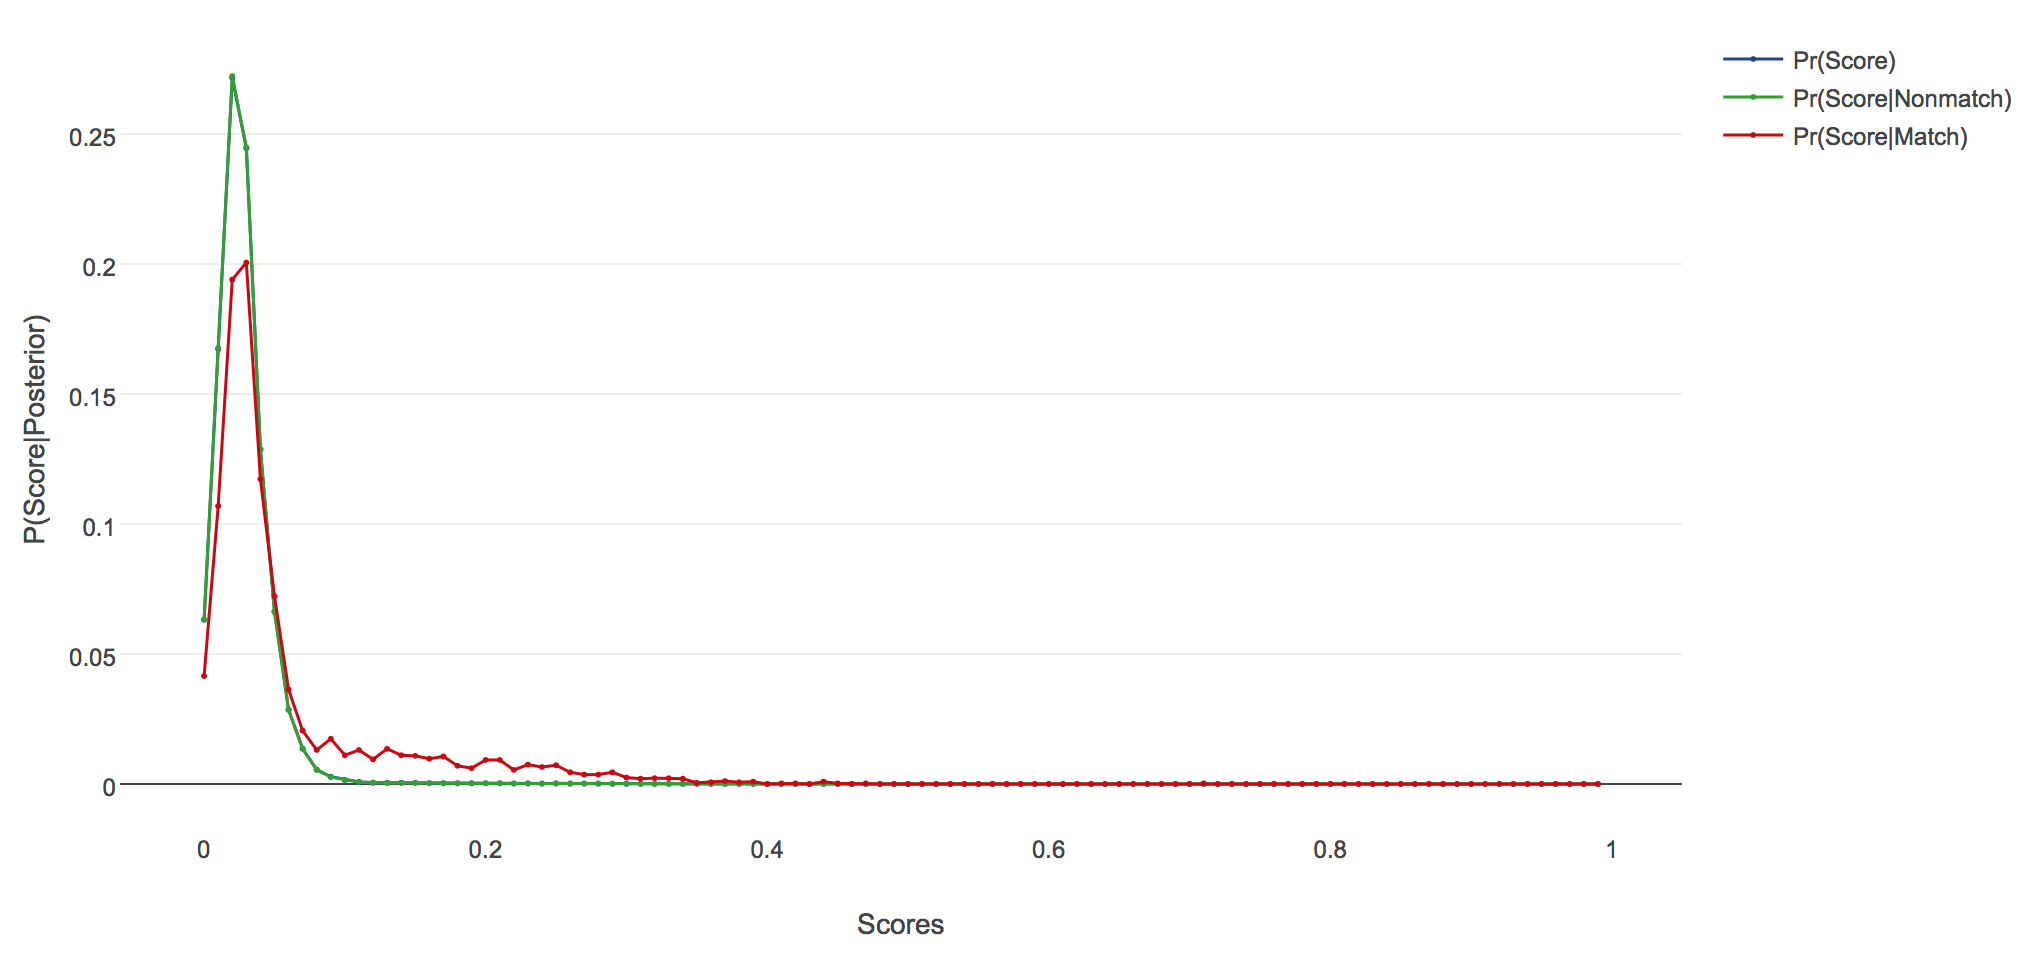
\includegraphics[width=0.95\textwidth]{dataset/grand/psm}}
  \label{fig:grand_psm}\\ %chktex 24
  \subfloat[][CDF of Score given matches/non-matches]
  {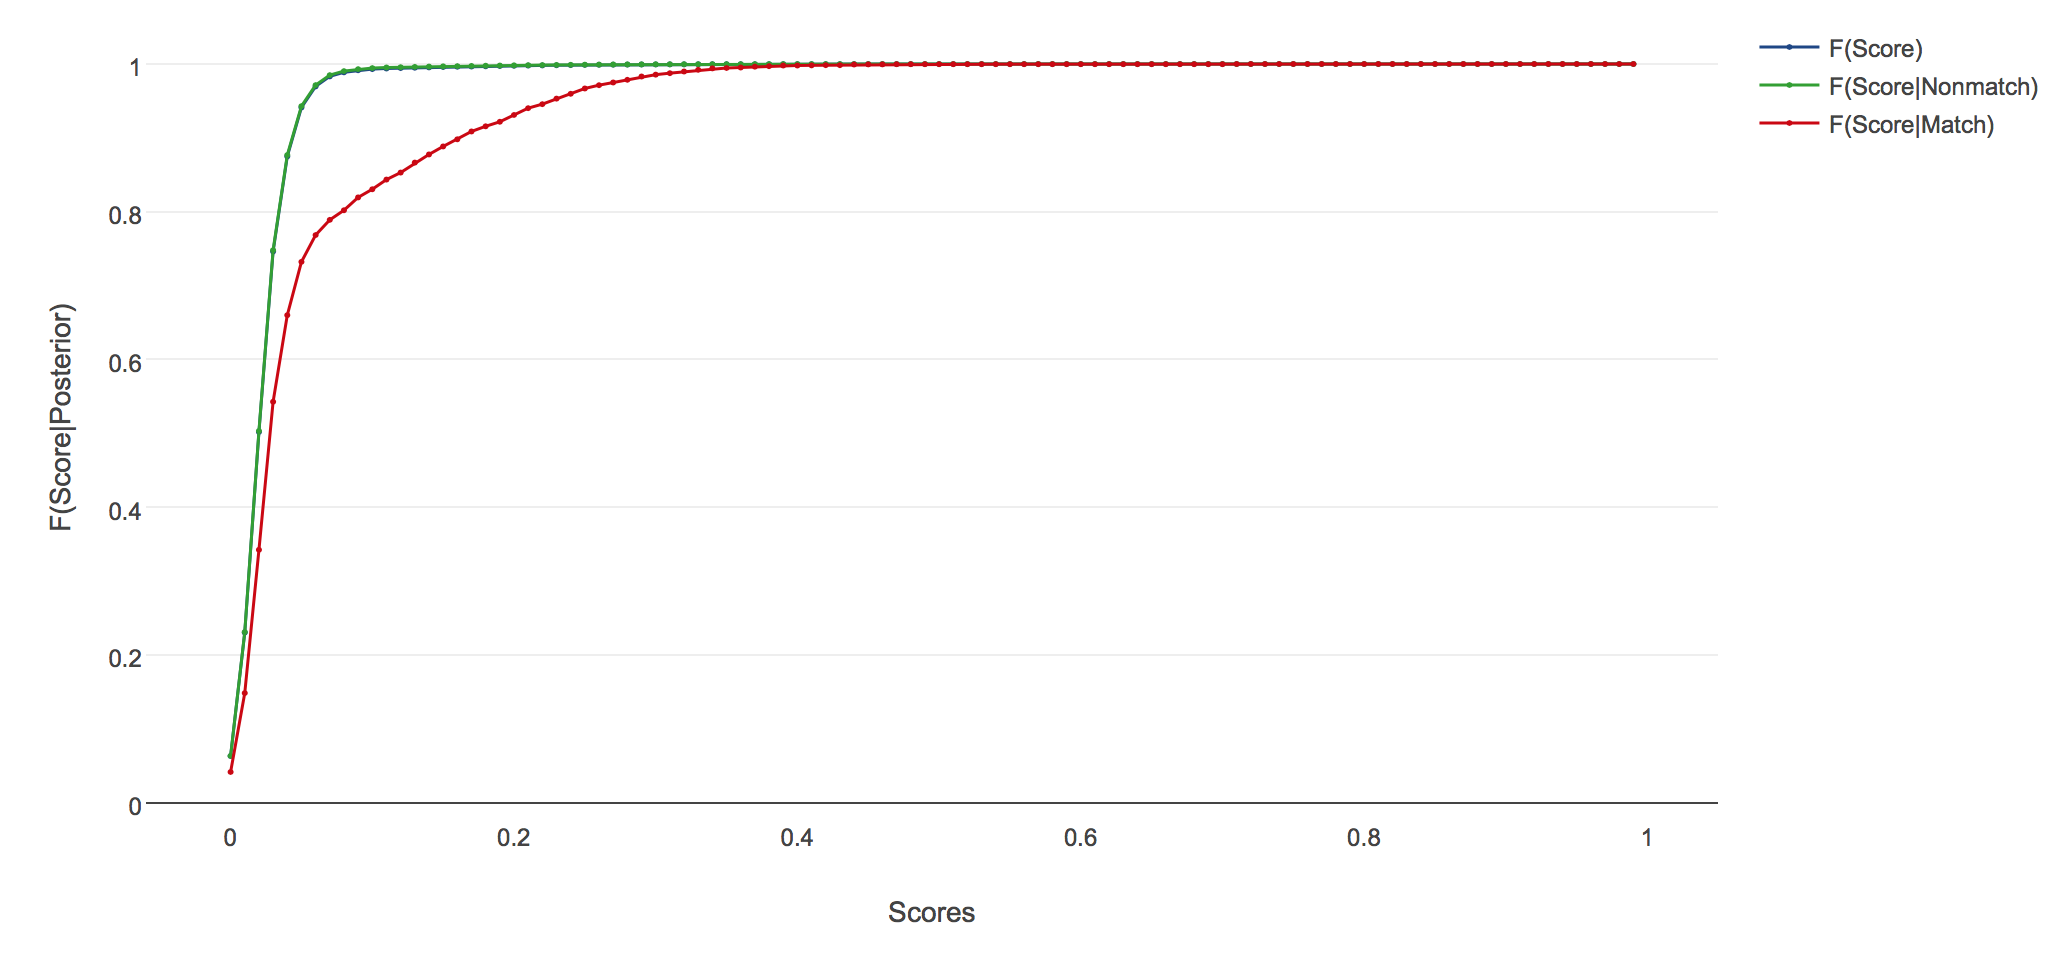
\includegraphics[width=0.95\textwidth]{dataset/grand/csm}}
  \label{fig:grand_csm}\\ %chktex 24
  \subfloat[][Difference between the CDF of Score given matches/non-matches]
  %$F\[non-match\]$ and $F\[match\]$
  {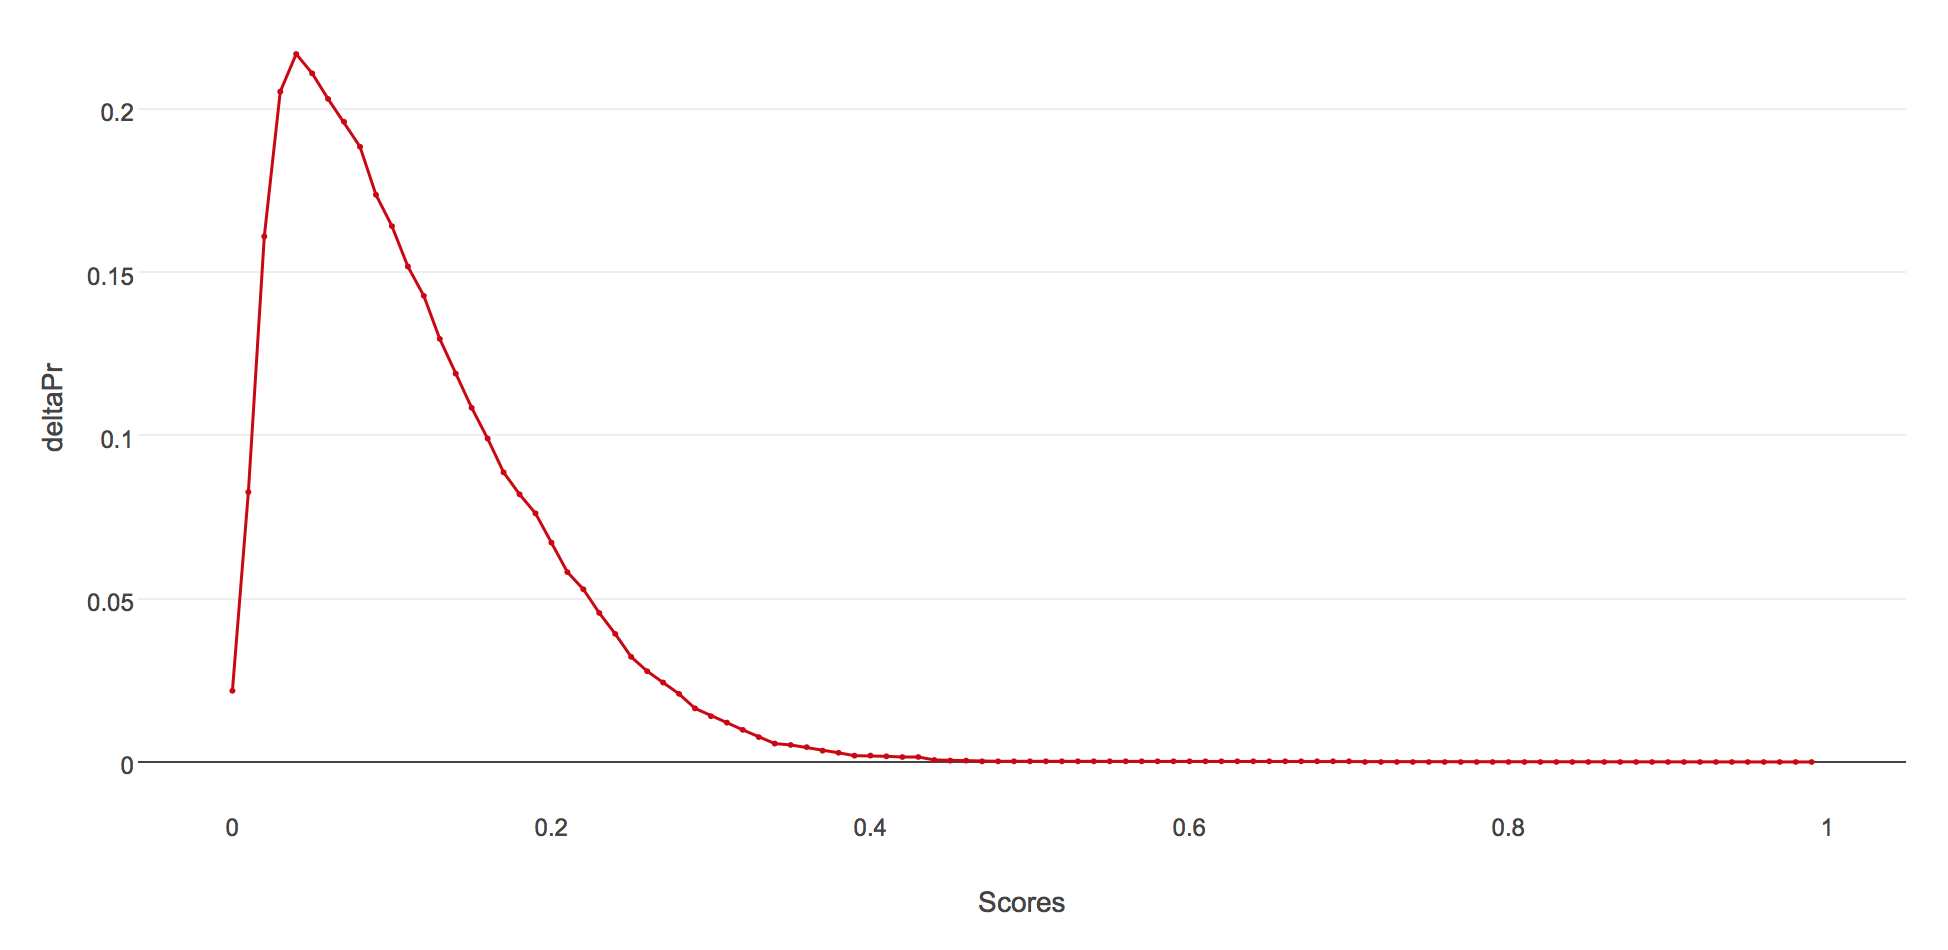
\includegraphics[width=0.95\textwidth]{dataset/grand/dsm}}
  \caption{Functions of Score given matches/non-matches}
  \label{fig:grand_dsm} %chktex 24
\end{figure}

From the plot above, we can deduct following conclusions:
\begin{itemize}
\item Most of the cohorts has score between 0 and 0.07 overall so most matches
and non-matches have score less than 0.06.
\item We expected $\Pr{(score \mid match)}$ to increase as the function of score
, but it turns out that it actually decreases. This results from the fact that
there are \emph{very few} matches with scores higher than 0.33, which is the 99th
percentile of the matches' score.
\item The number of matches with $score \in [0.08, 0.35)$ is greater than that of
non-matches with the score in the same range. That is
$$\Pr{(score \mid match)} > \Pr{(score \mid nonmatch)} \mbox{ where } score\in [0.08, 0.35)$$
\end{itemize}

\begin{figure}[h!]
  \centering
  \subfloat[][Probability of Score given matches/non-matches]
  {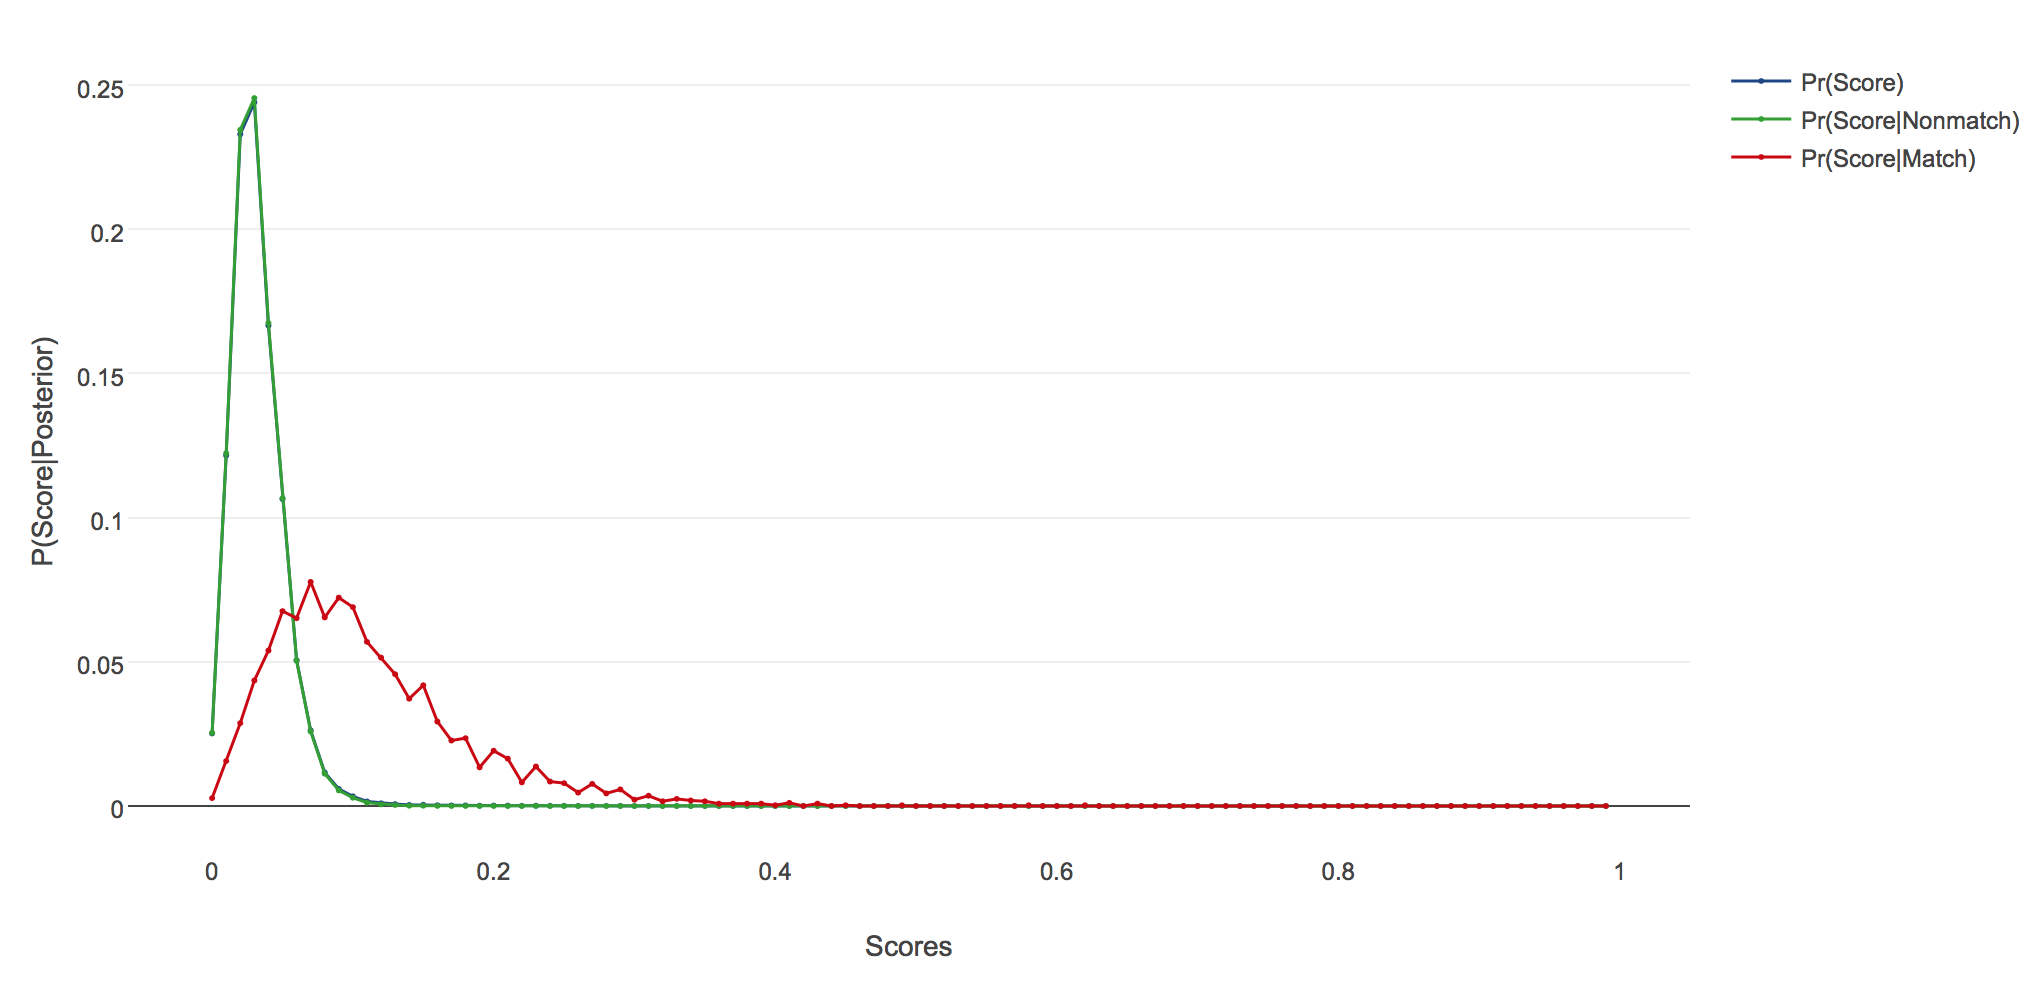
\includegraphics[width=0.95\textwidth]{dataset/otago/psm}}
  \label{fig:otago_psm}\\ %chktex 24
  \subfloat[][CDF of Score given matches/non-matches]
  {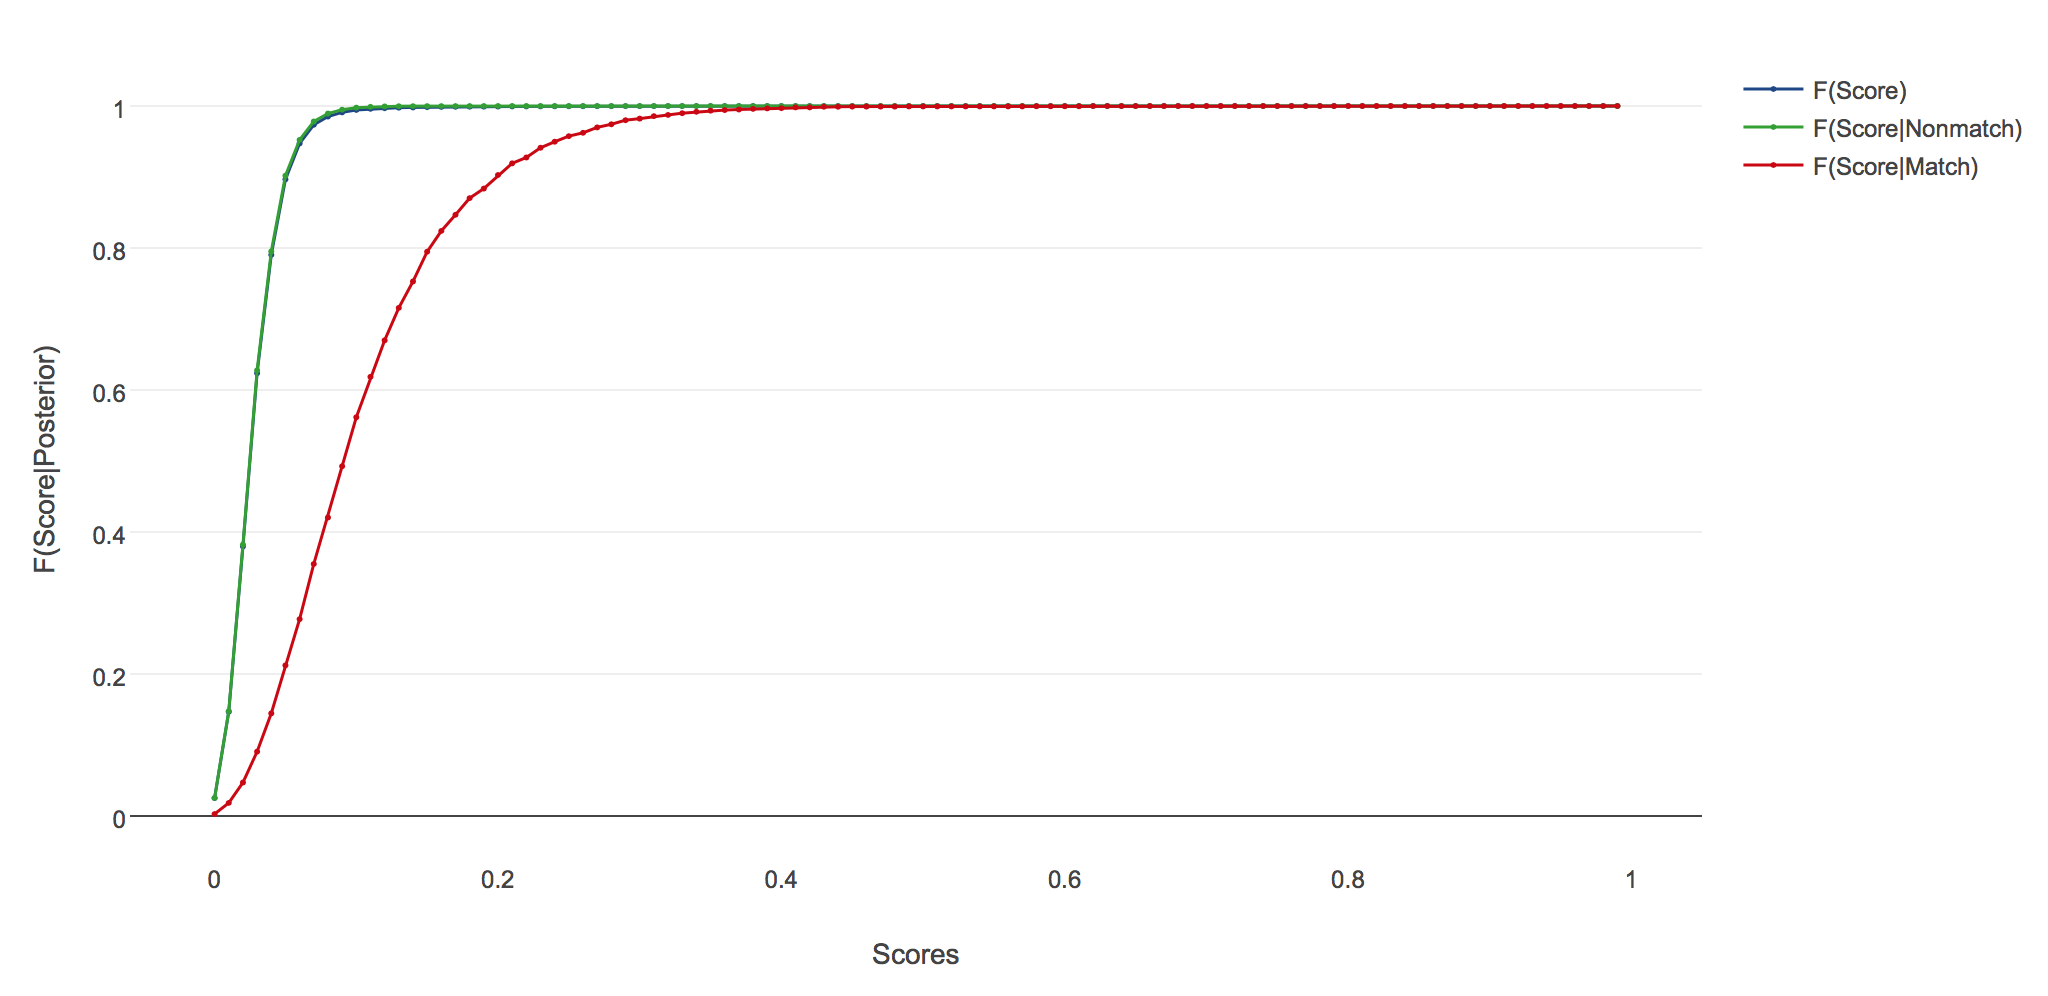
\includegraphics[width=0.95\textwidth]{dataset/otago/csm}}
  \label{fig:otago_csm}\\ %chktex 24
  \subfloat[][Difference between the CDF of Score given matches/non-matches]
    %$F\[non-match\]$ and $F\[match\]$
  {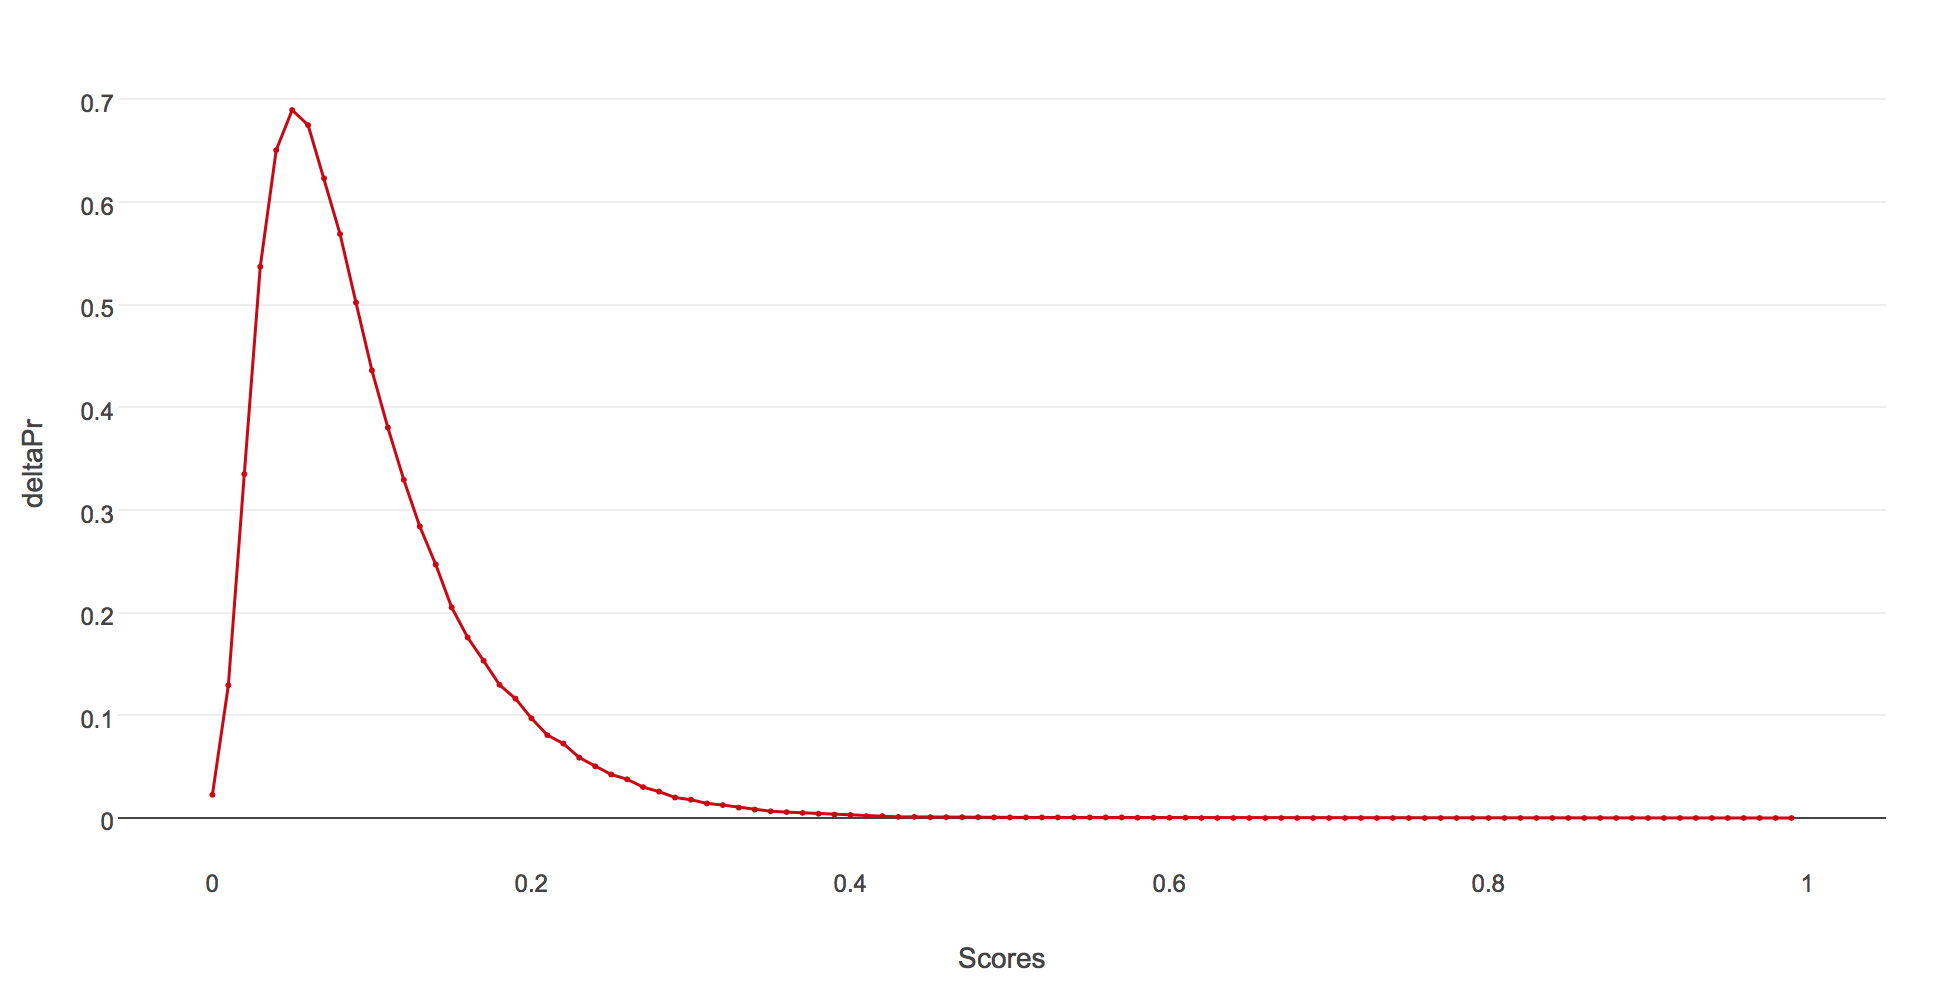
\includegraphics[width=0.95\textwidth]{dataset/otago/dsm}}
  \caption{Functions of Score given matches/non-matches}
  \label{fig:otago_dsm} %chktex 24
\end{figure}


\subsection{Probability of a matching score at a given cohort size}

\begin{figure}[ht]
  \centering
  \subfloat[][Probability of a matching score at a given cohort size]
  {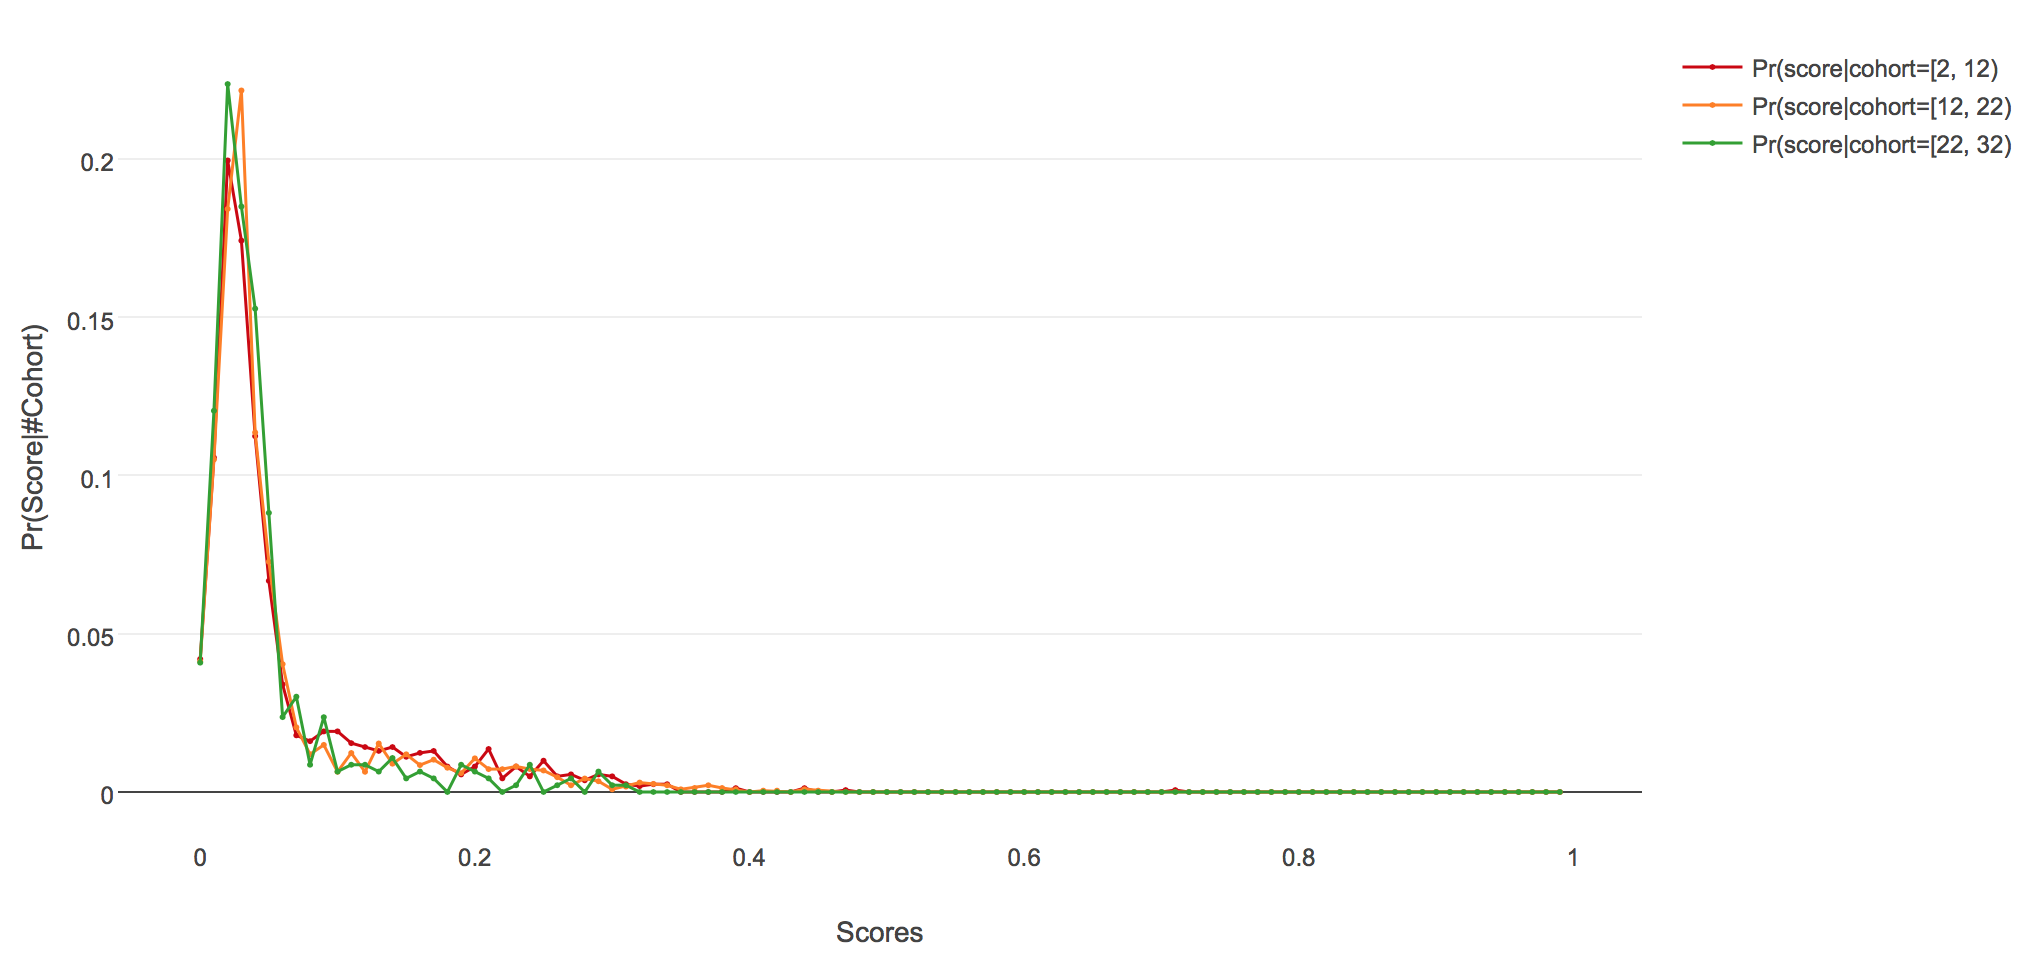
\includegraphics[width=0.95\textwidth]{dataset/grand/pscohort}}
  \label{fig:grand_pscohort}\\ %chktex 24
  \subfloat[][Probability of a score \emph{not} in a given cohort size]
  {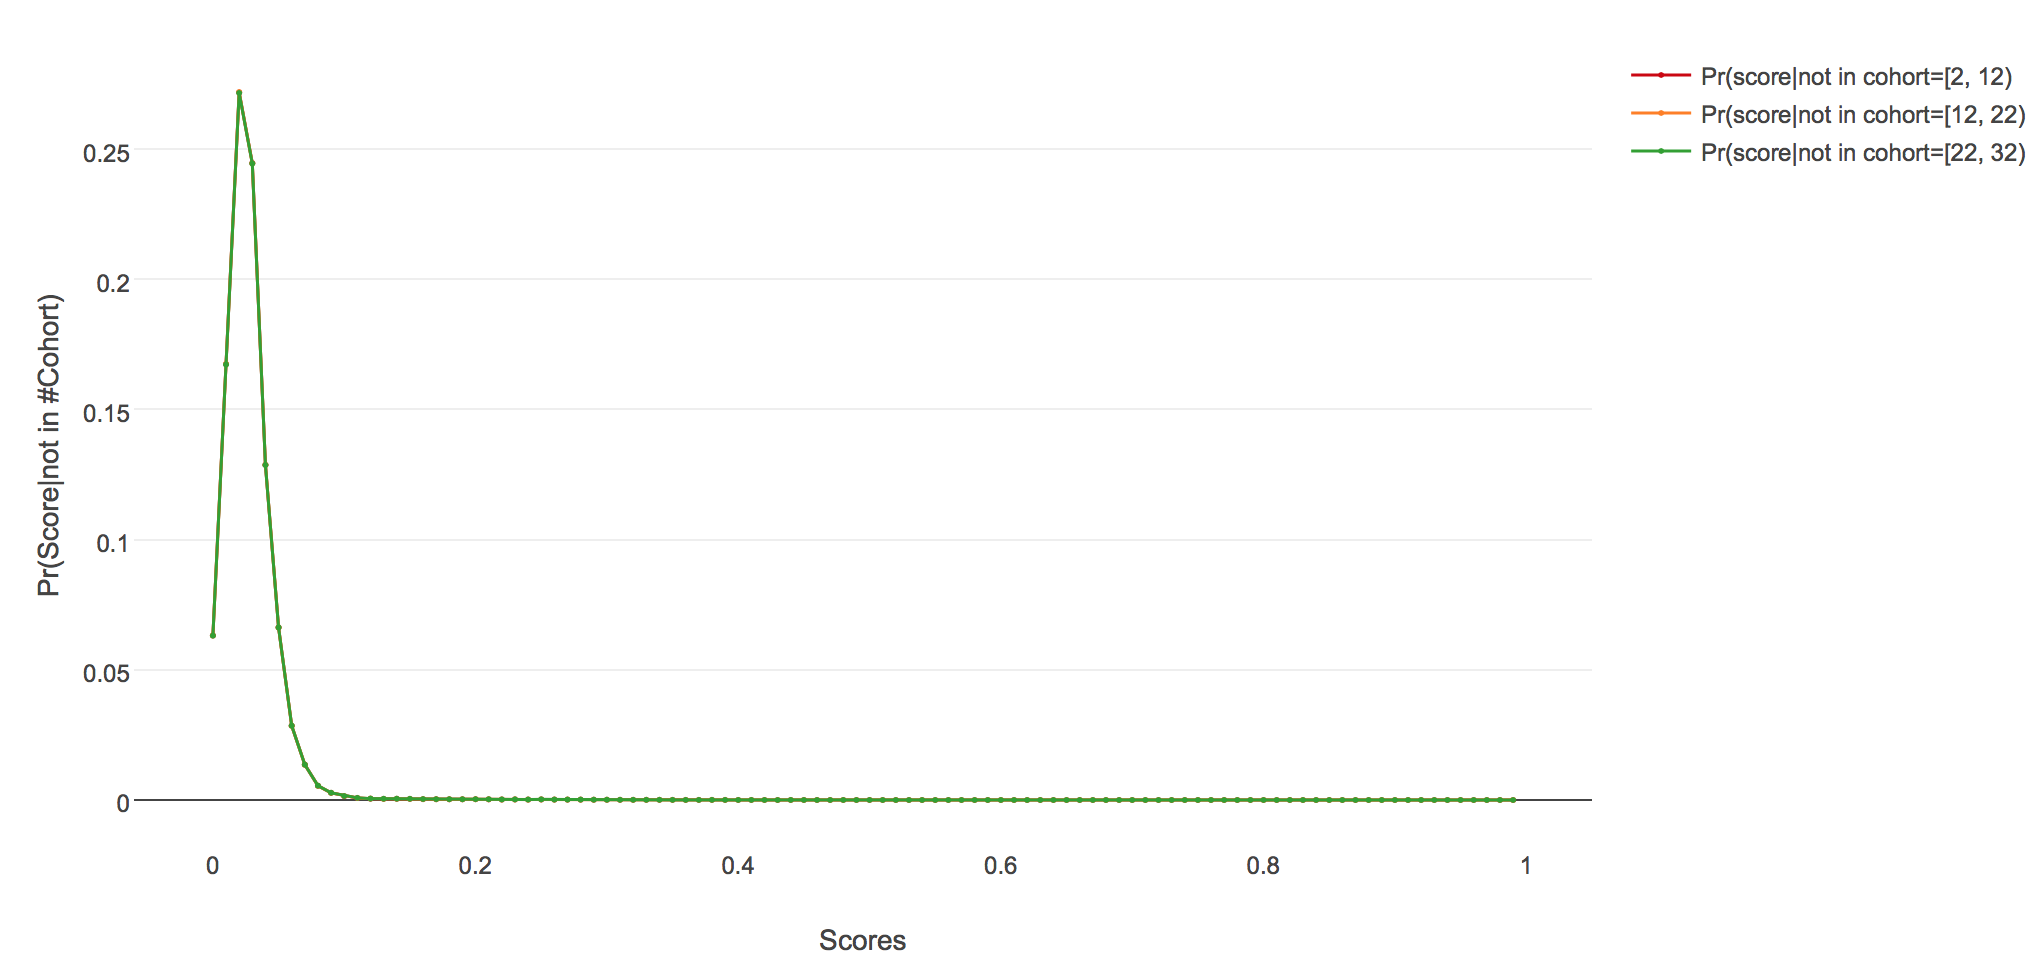
\includegraphics[width=0.95\textwidth]{dataset/grand/psnoncohort}}
  \caption{Probability of a score given a range of cohort size}
  \label{fig:grand_psnoncohort} %chktex 24
\end{figure}

Initially, we expected that as the cohort size increases, $\Pr{(score \mid
\#cohort)}$ should peak closer to 1 since $\texttt{selfscore}$ should decrease
and $\max{(\texttt{sift\_match}(I_i, I_j))}$ should increase as the number of
captures in a cohort increases. However, the distribution of $\Pr{(score \mid
\#cohort)}$ for all numbers of cohorts seem to be similar to one another.

\begin{figure}[ht]
  \centering
  \subfloat[][Probability of a matching score at a given cohort size]
  {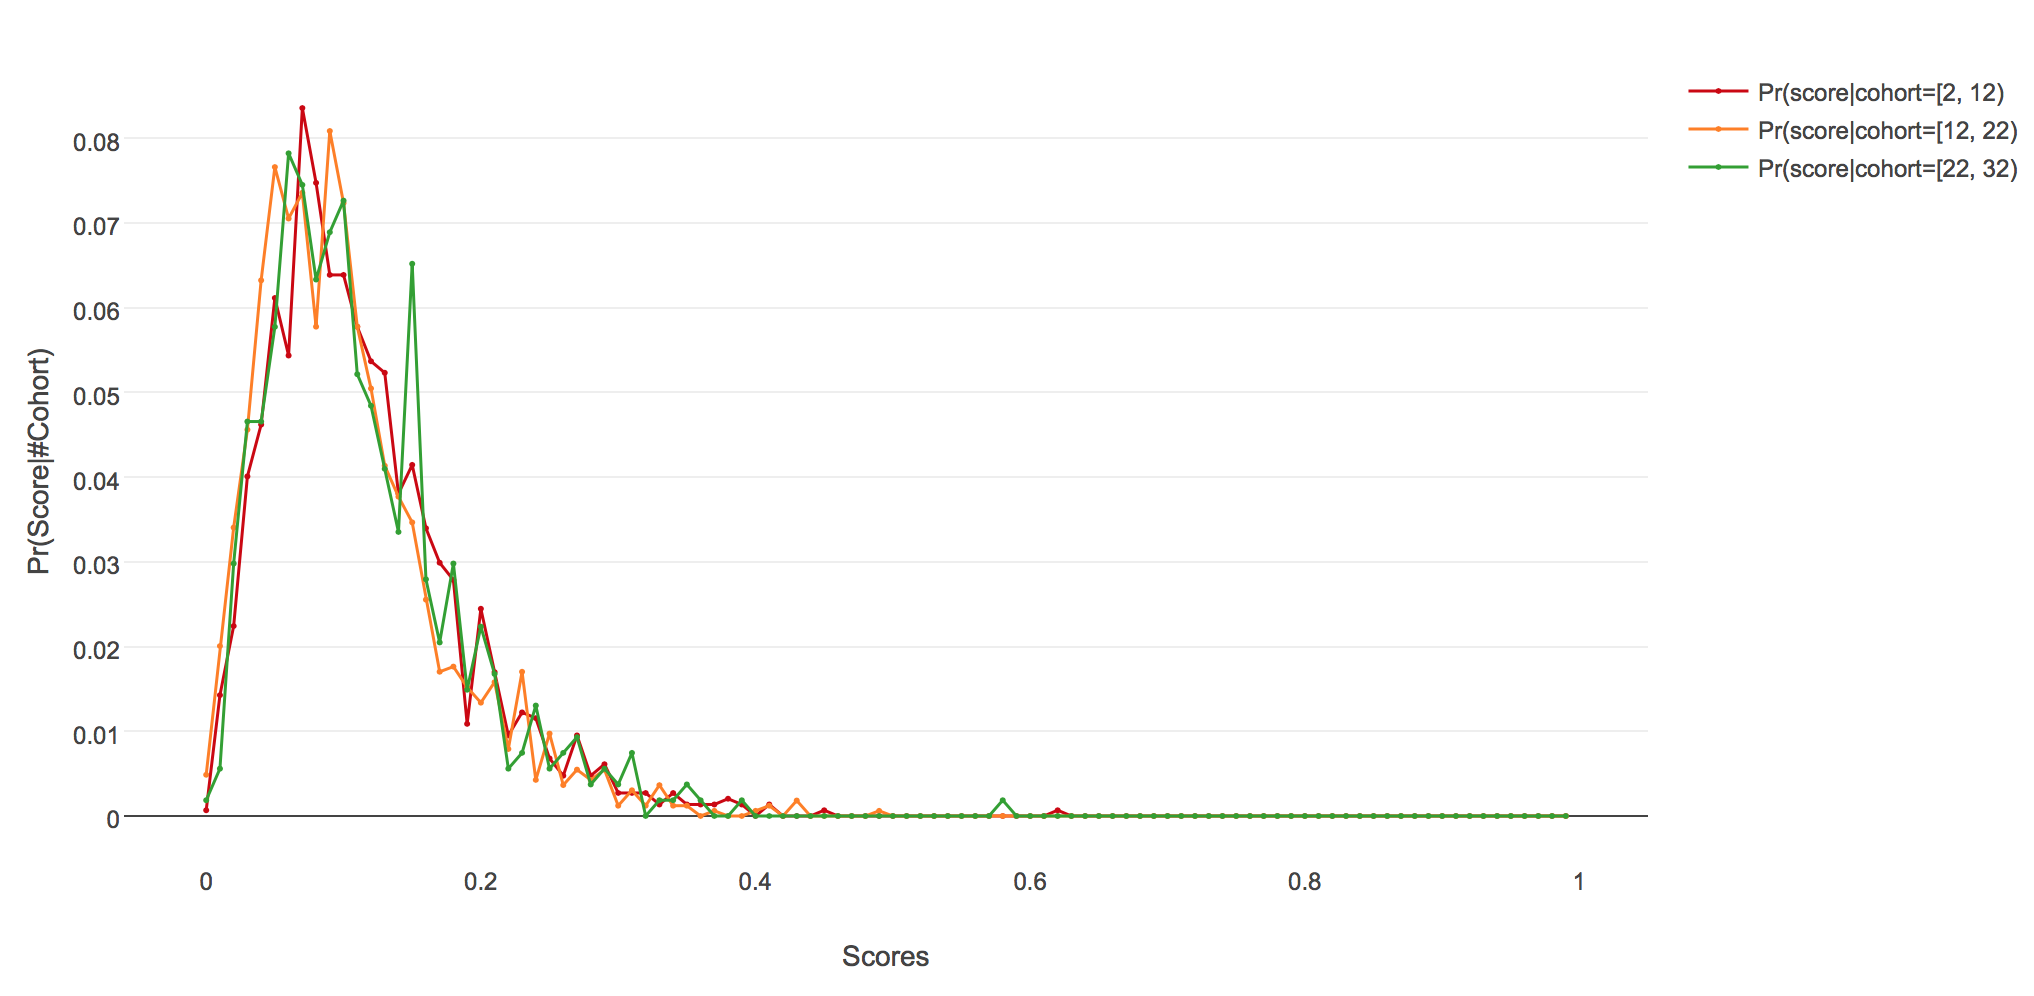
\includegraphics[width=0.95\textwidth]{dataset/otago/pscohort}}
  \label{fig:otago_pscohort}\\ %chktex 24
  \subfloat[][Probability of a score \emph{not} in a given cohort size]
  {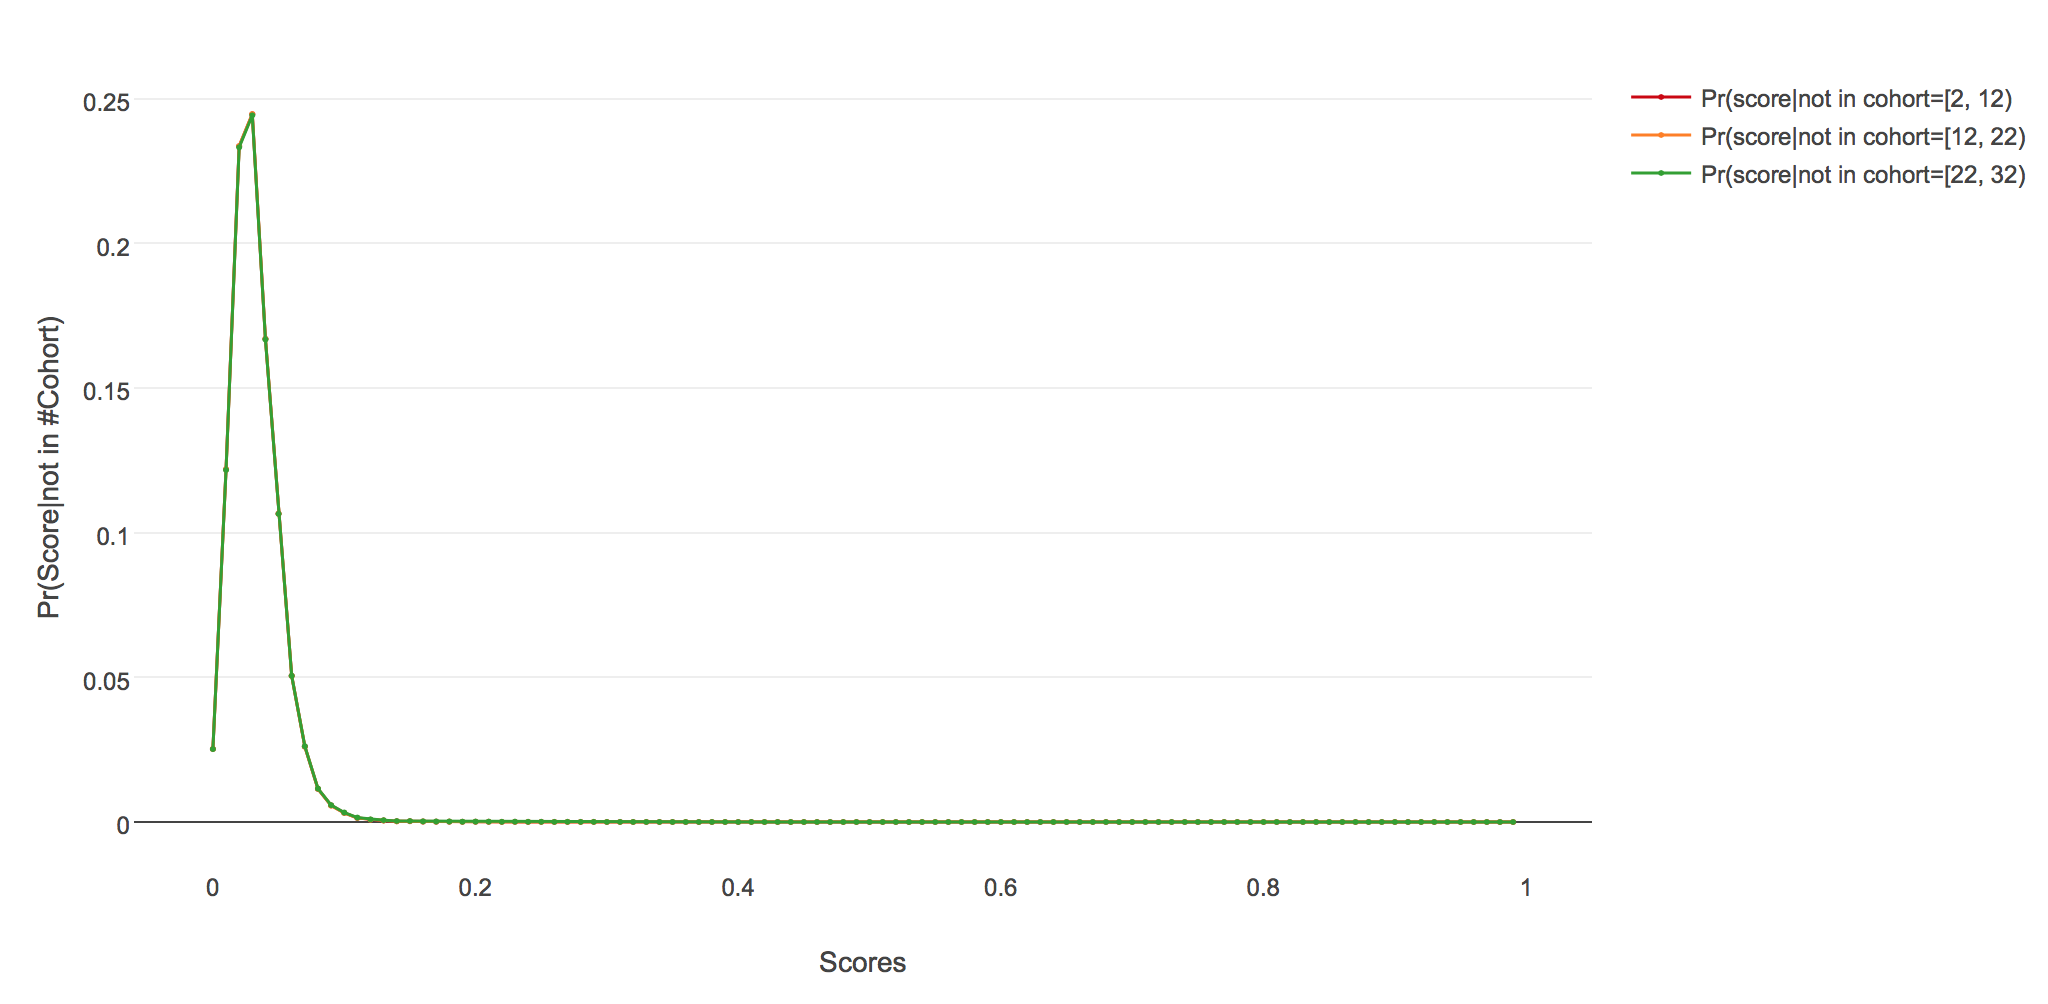
\includegraphics[width=0.95\textwidth]{dataset/otago/psnoncohort}}
  \caption{Probability of a score given a range of cohort size}
  \label{fig:otago_psnoncohort} %chktex 24
\end{figure}

\subsection{Earth Mover's Distance}

We use Earth Mover's Distance (EMD)~\cite{emd00} as our metric to calculate the
minimal cost required to transform $\Pr{(score \mid nonmatch)}$ to $\Pr{(score \mid match)}$.

\begin{figure}[ht]
  \centering
  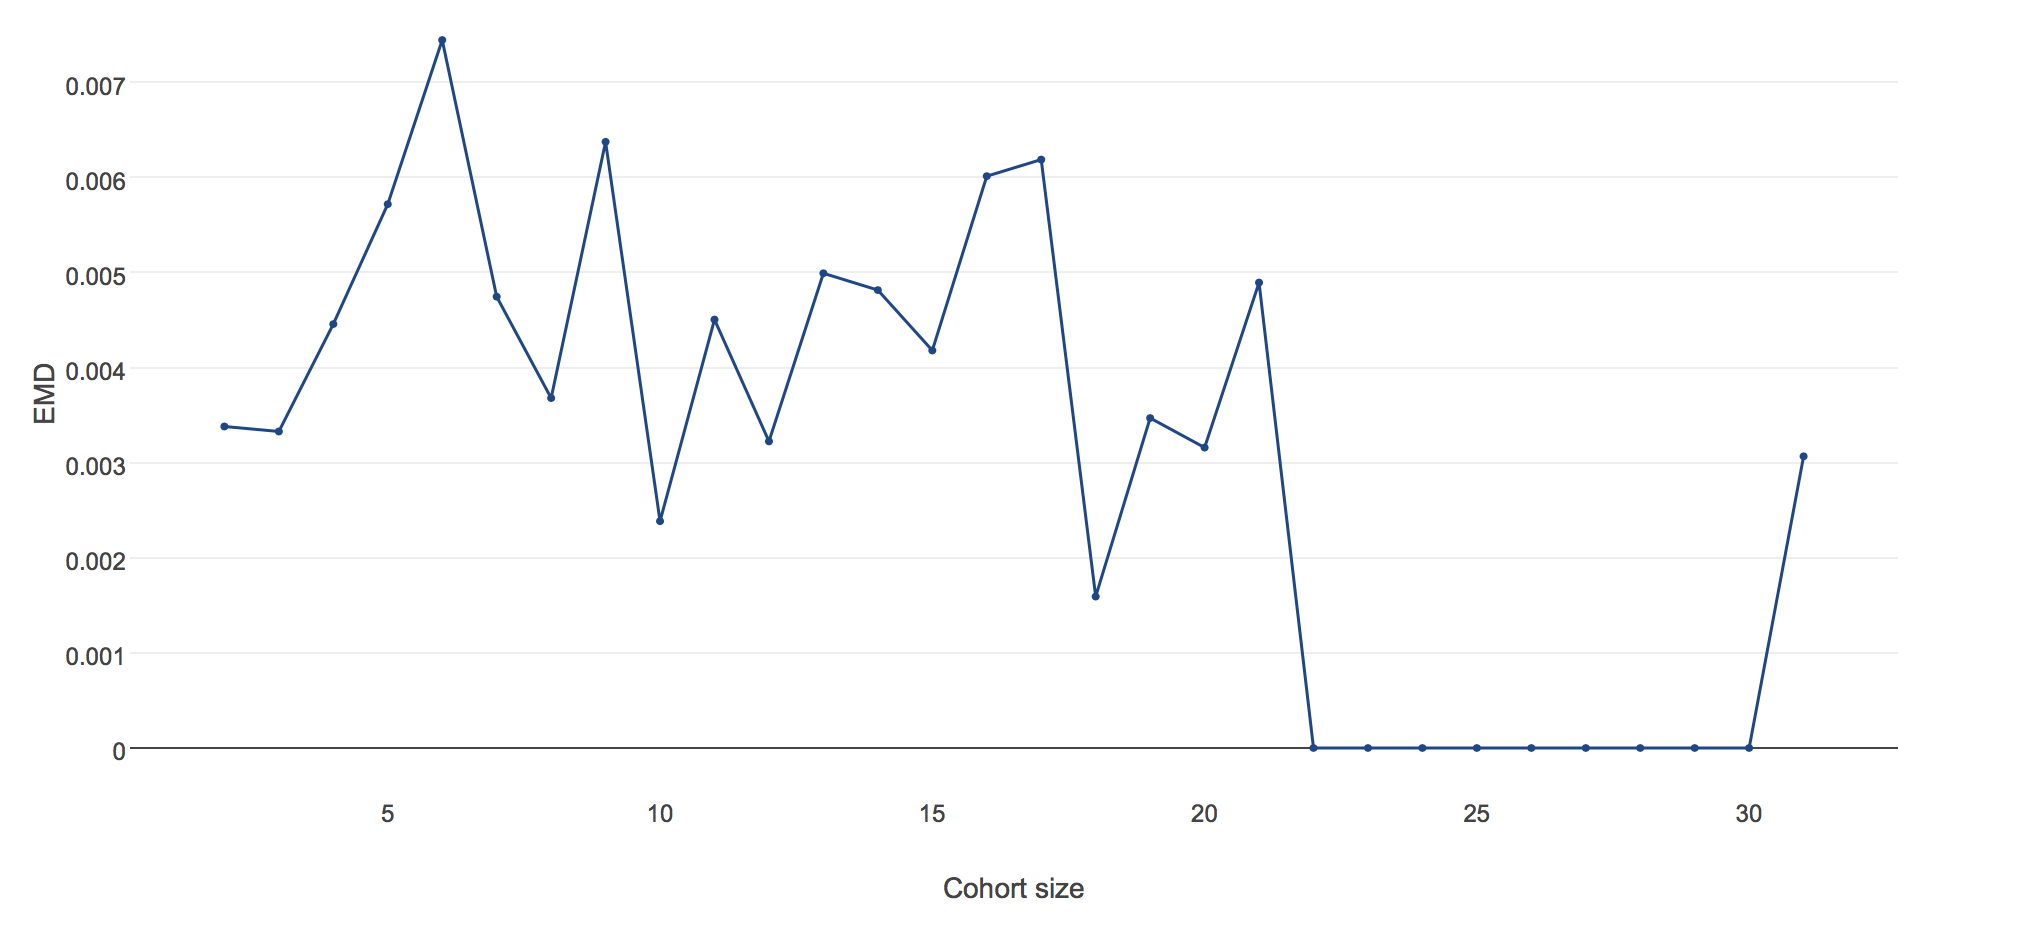
\includegraphics[width=0.95\textwidth]{dataset/grand/emd}
  \caption{Earth Mover's Distance between the probability distributions}
  \label{fig:grand_emd} %chktex 24
\end{figure}

Initially, we also expected that the relationship between EMD and cohort size
should be Gaussian. However, there seem to be no relationship between
$\Pr{(score \mid nonmatch)}$ and $\Pr{(score \mid match)}$.

\begin{figure}[ht]
  \centering
  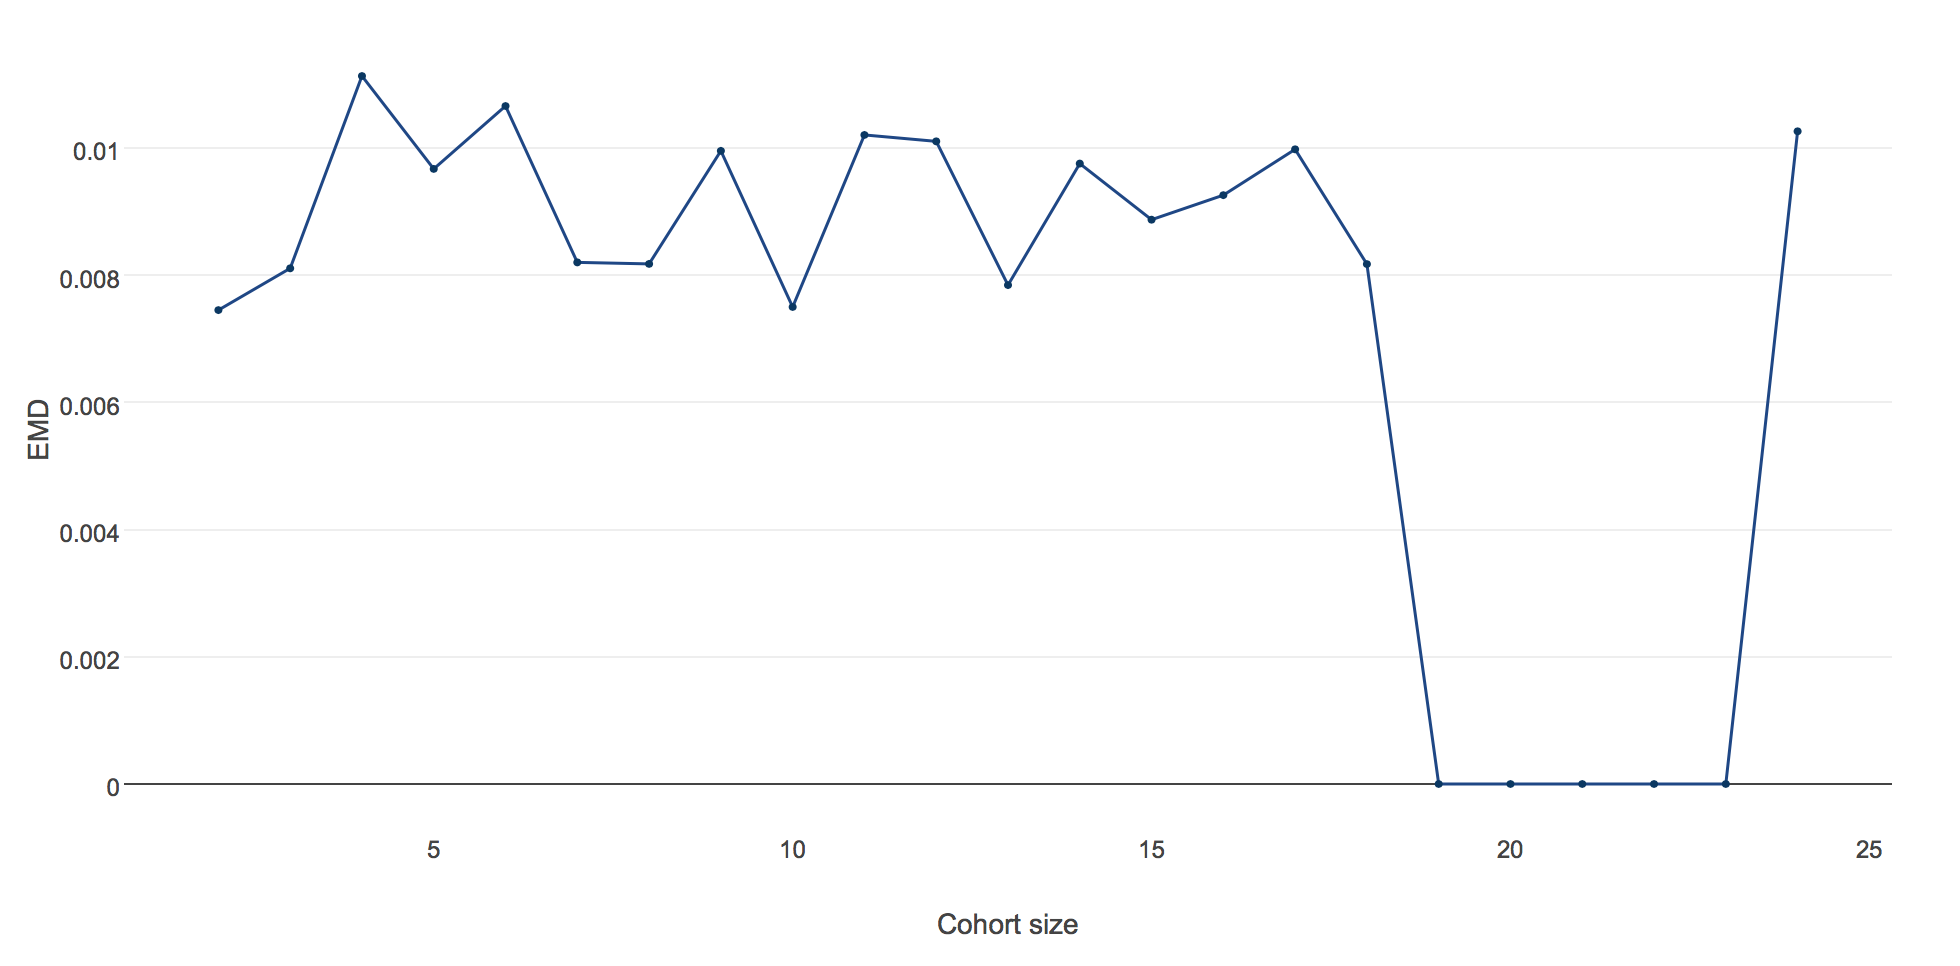
\includegraphics[width=0.95\textwidth]{dataset/otago/emd}
  \caption{Earth Mover's Distance between the probability distributions}
  \label{fig:otago_emd} %chktex 24
\end{figure}

\subsection{Entropy of $\Pr{(score \mid match)}$ at different cohort sizes}

Entropy is the average amount of information we get from each distribution.
$H(X|Y)$ = amount of randomness in the random variable X given the event Y.

\begin{figure}[ht]
  \centering
  \subfloat[][Entropy of $\Pr{(score \mid match)}$ at different cohort sizes]
  {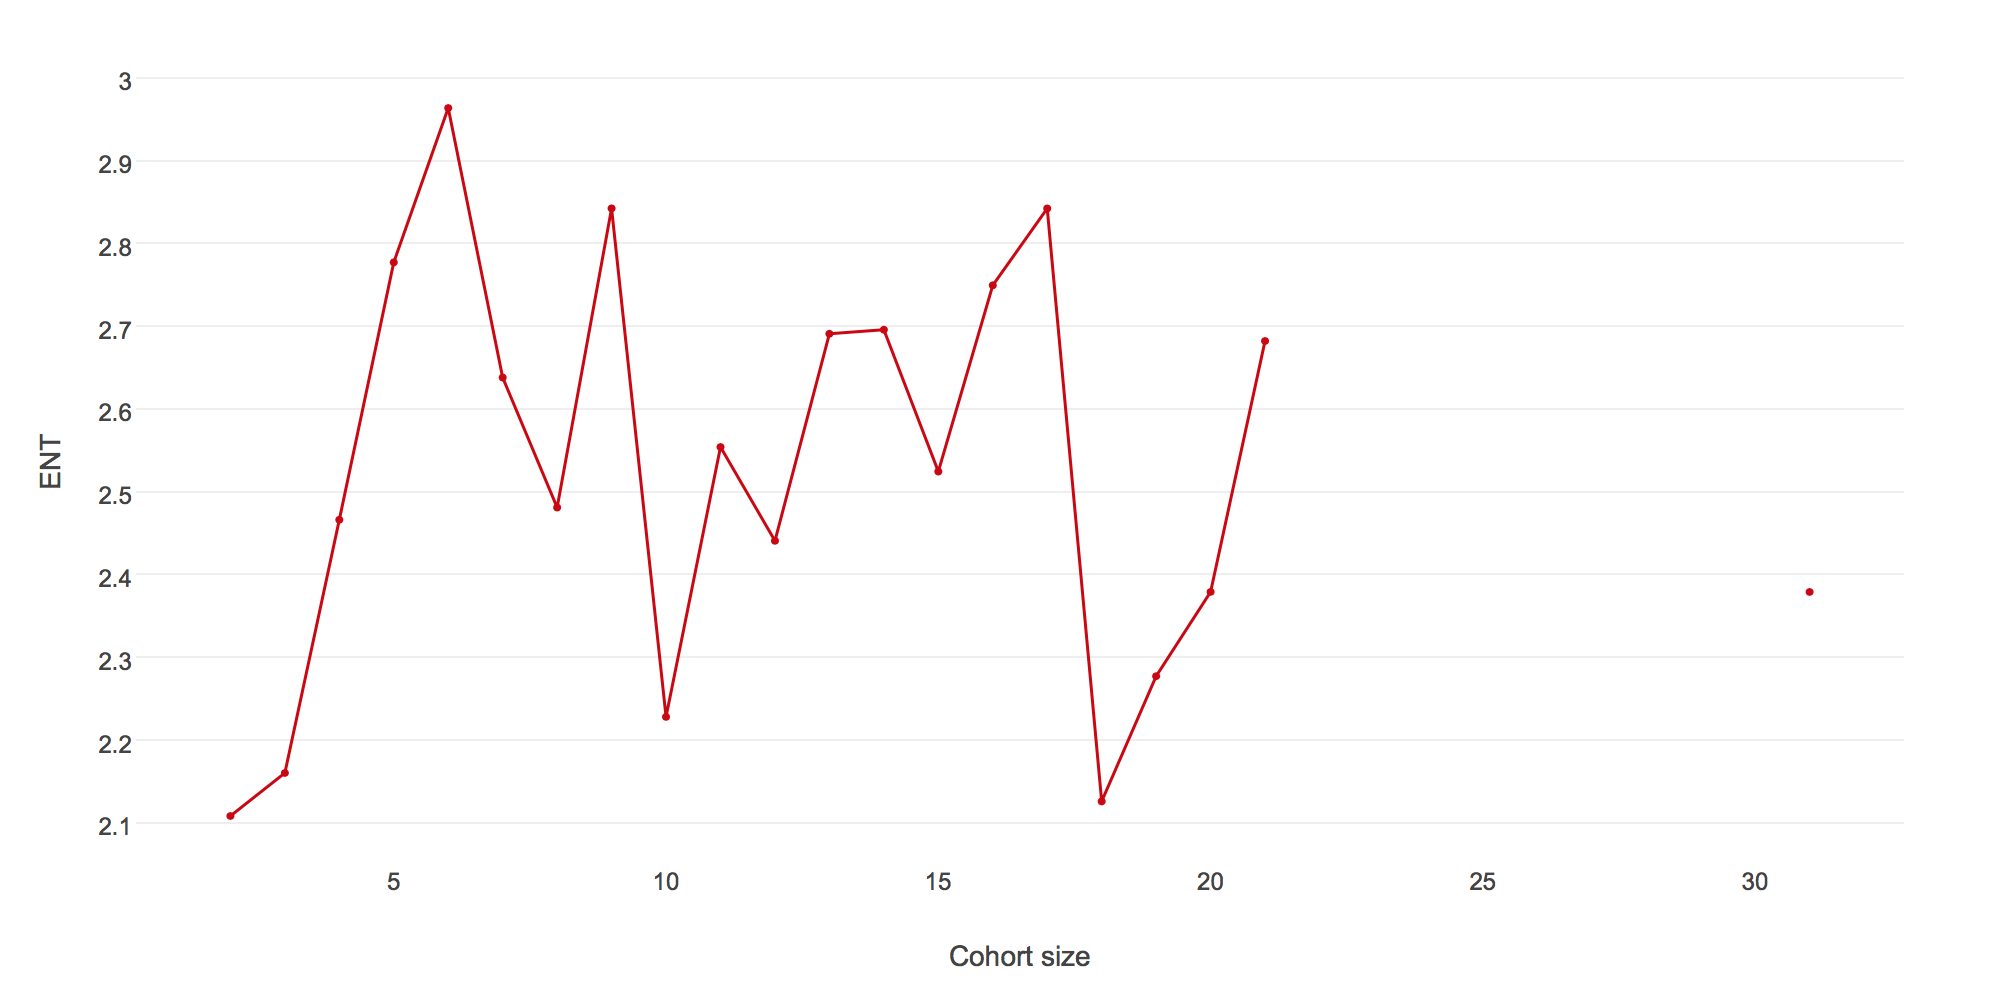
\includegraphics[width=0.95\textwidth]{dataset/grand/ent_psm}}
  \label{fig:grand_ent_psm}\\ %chktex 24
  \subfloat[][Entropy of $\Pr{(score \mid nonmatch)}$ at different cohort sizes]
  {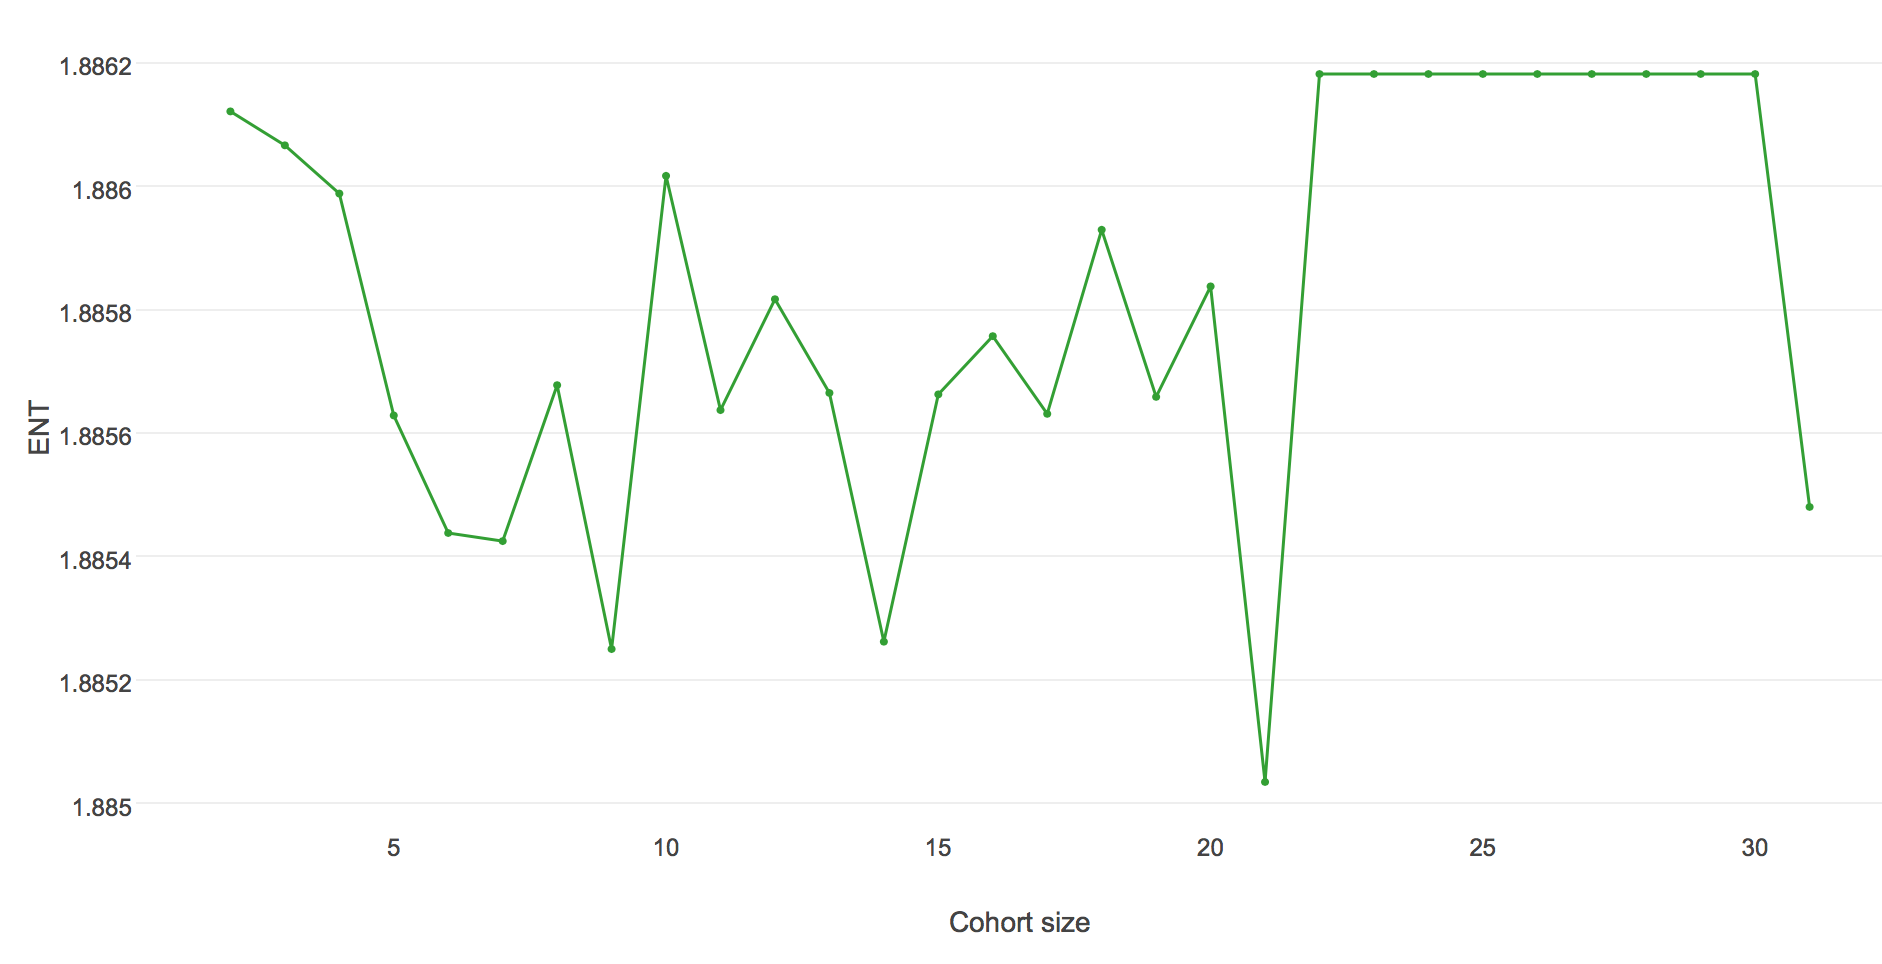
\includegraphics[width=0.95\textwidth]{dataset/grand/ent_psnm}}
  \caption{Relationship between $\Pr{(score \mid match)}$ and $\Pr{(score \mid nonmatch)}$}
  \label{fig:grand_ent_psnm} %chktex 24
\end{figure}

\begin{figure}[ht]
  \centering
  \subfloat[][Entropy of $\Pr{(score \mid match)}$ at different cohort sizes]
  {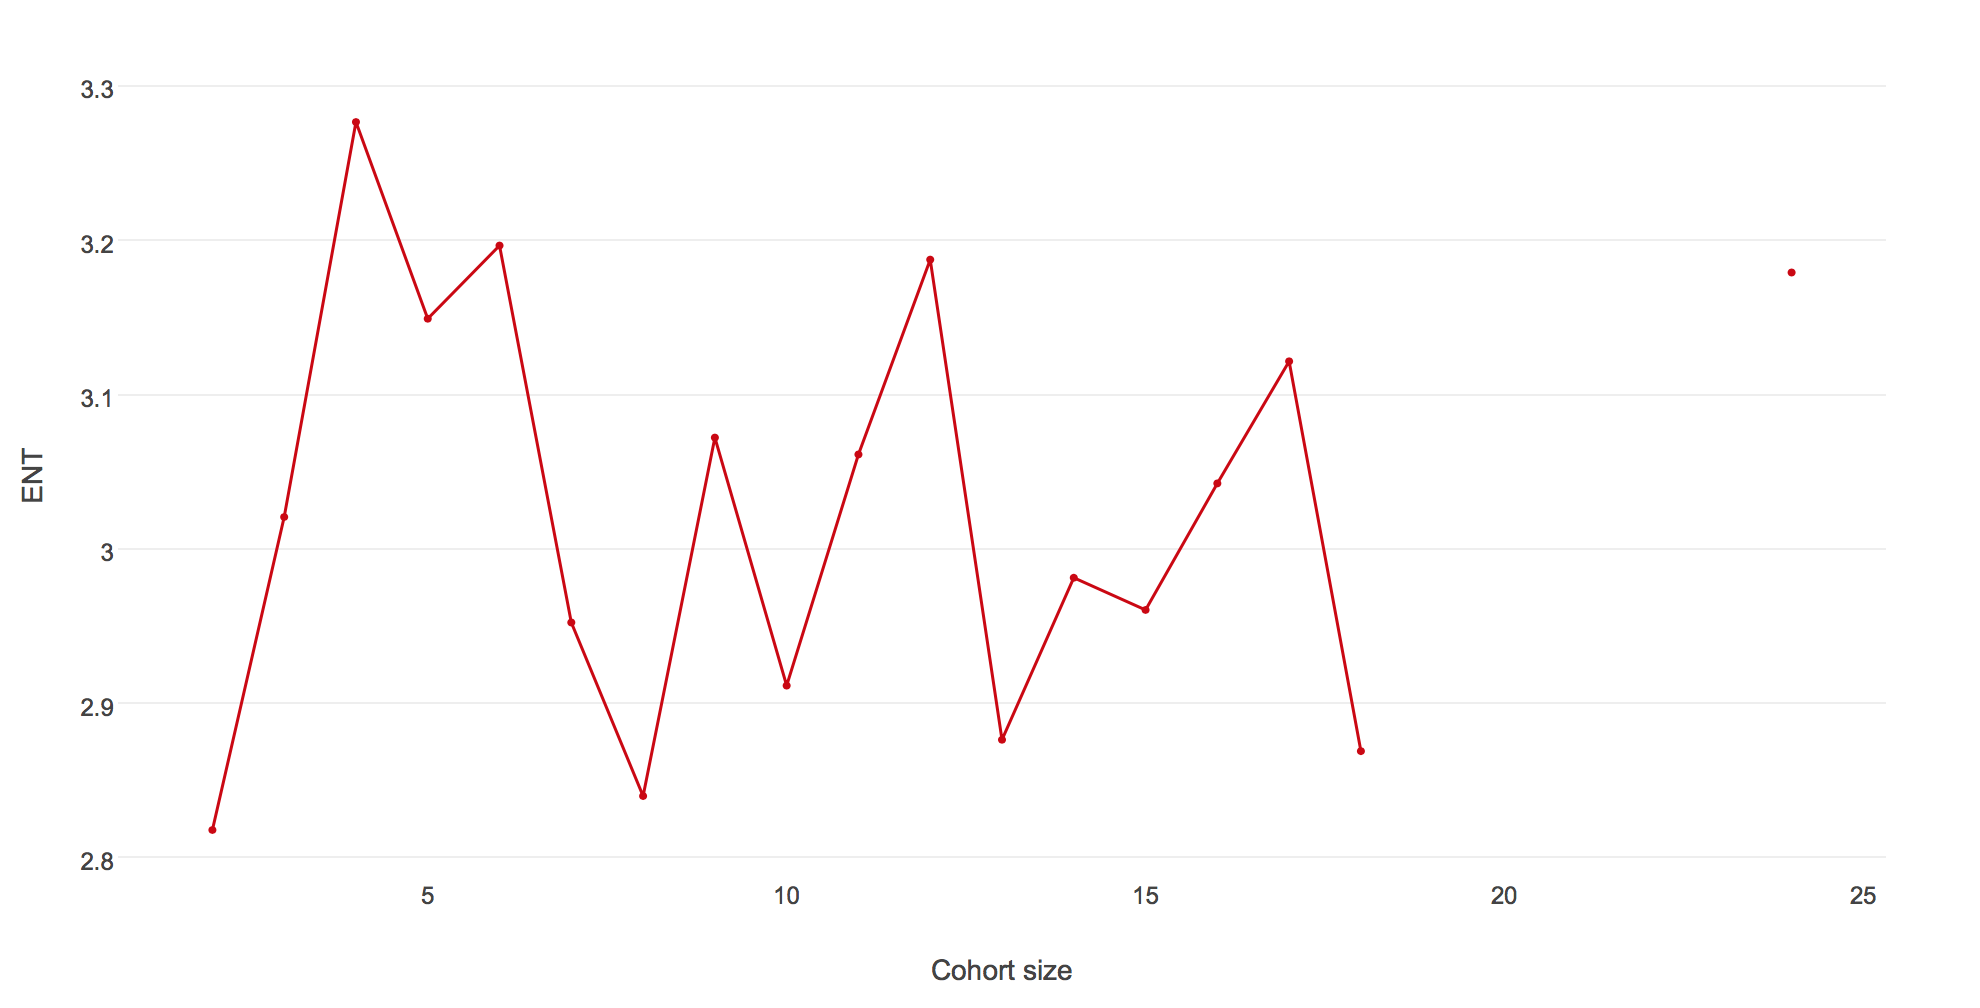
\includegraphics[width=0.95\textwidth]{dataset/otago/ent_psm}}
  \label{fig:otago_ent_psm}\\ %chktex 24
  \subfloat[][Entropy of $\Pr{(score \mid nonmatch)}$ at different cohort sizes]
  {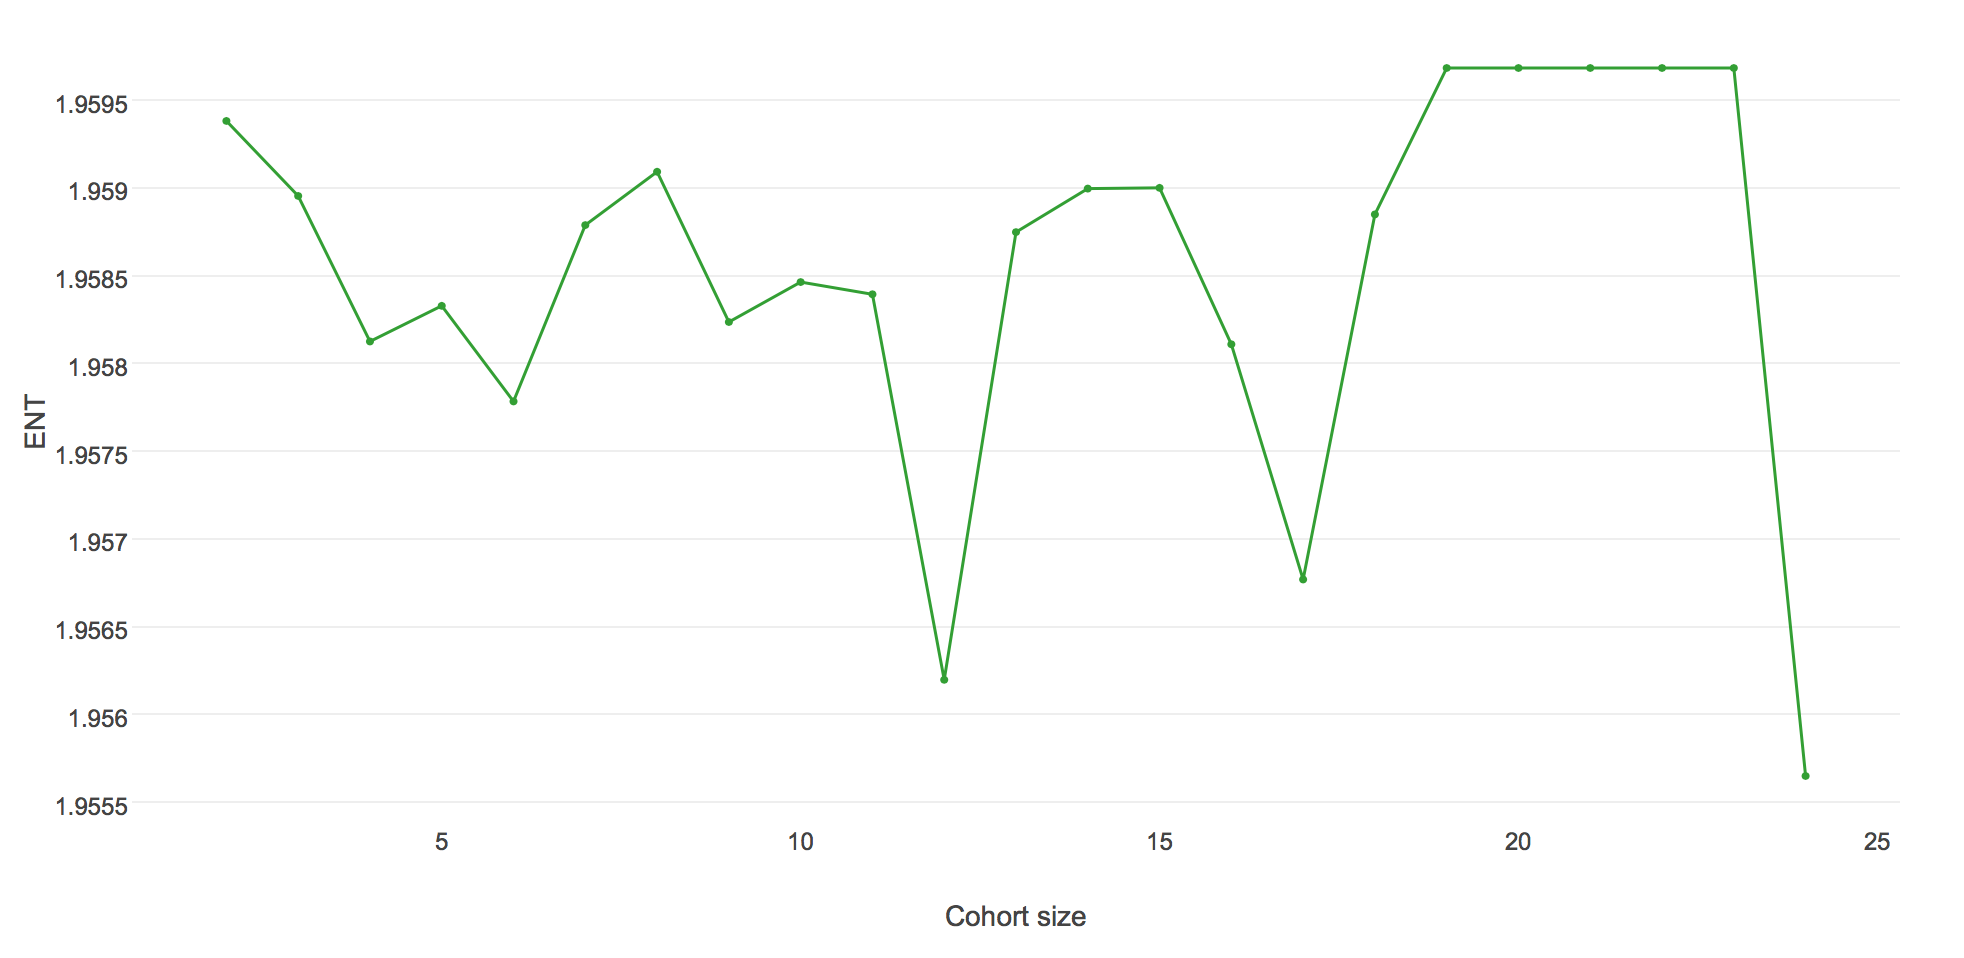
\includegraphics[width=0.95\textwidth]{dataset/otago/ent_psnm}}
  \label{fig:otago_ent_psnm}\\ %chktex 24
  \caption{Relationship between $\Pr{(score \mid match)}$ and $\Pr{(score \mid nonmatch)}$}
  \label{fig:emd_grand} %chktex 24
\end{figure}

\subsection{Probability of a Matches/Non-matches}

$$\Pr{(match \mid score)} = \frac{\Pr{(score \mid match)}\Pr{(match)}}
    {\Pr{(score)}}$$

$$\Pr{(nonmatch \mid score)} = \frac{\Pr{(score \mid nonmatch)}\Pr{(nonmatch)}}
    {\Pr{(score)}}$$

\begin{figure}[ht]
  \centering
  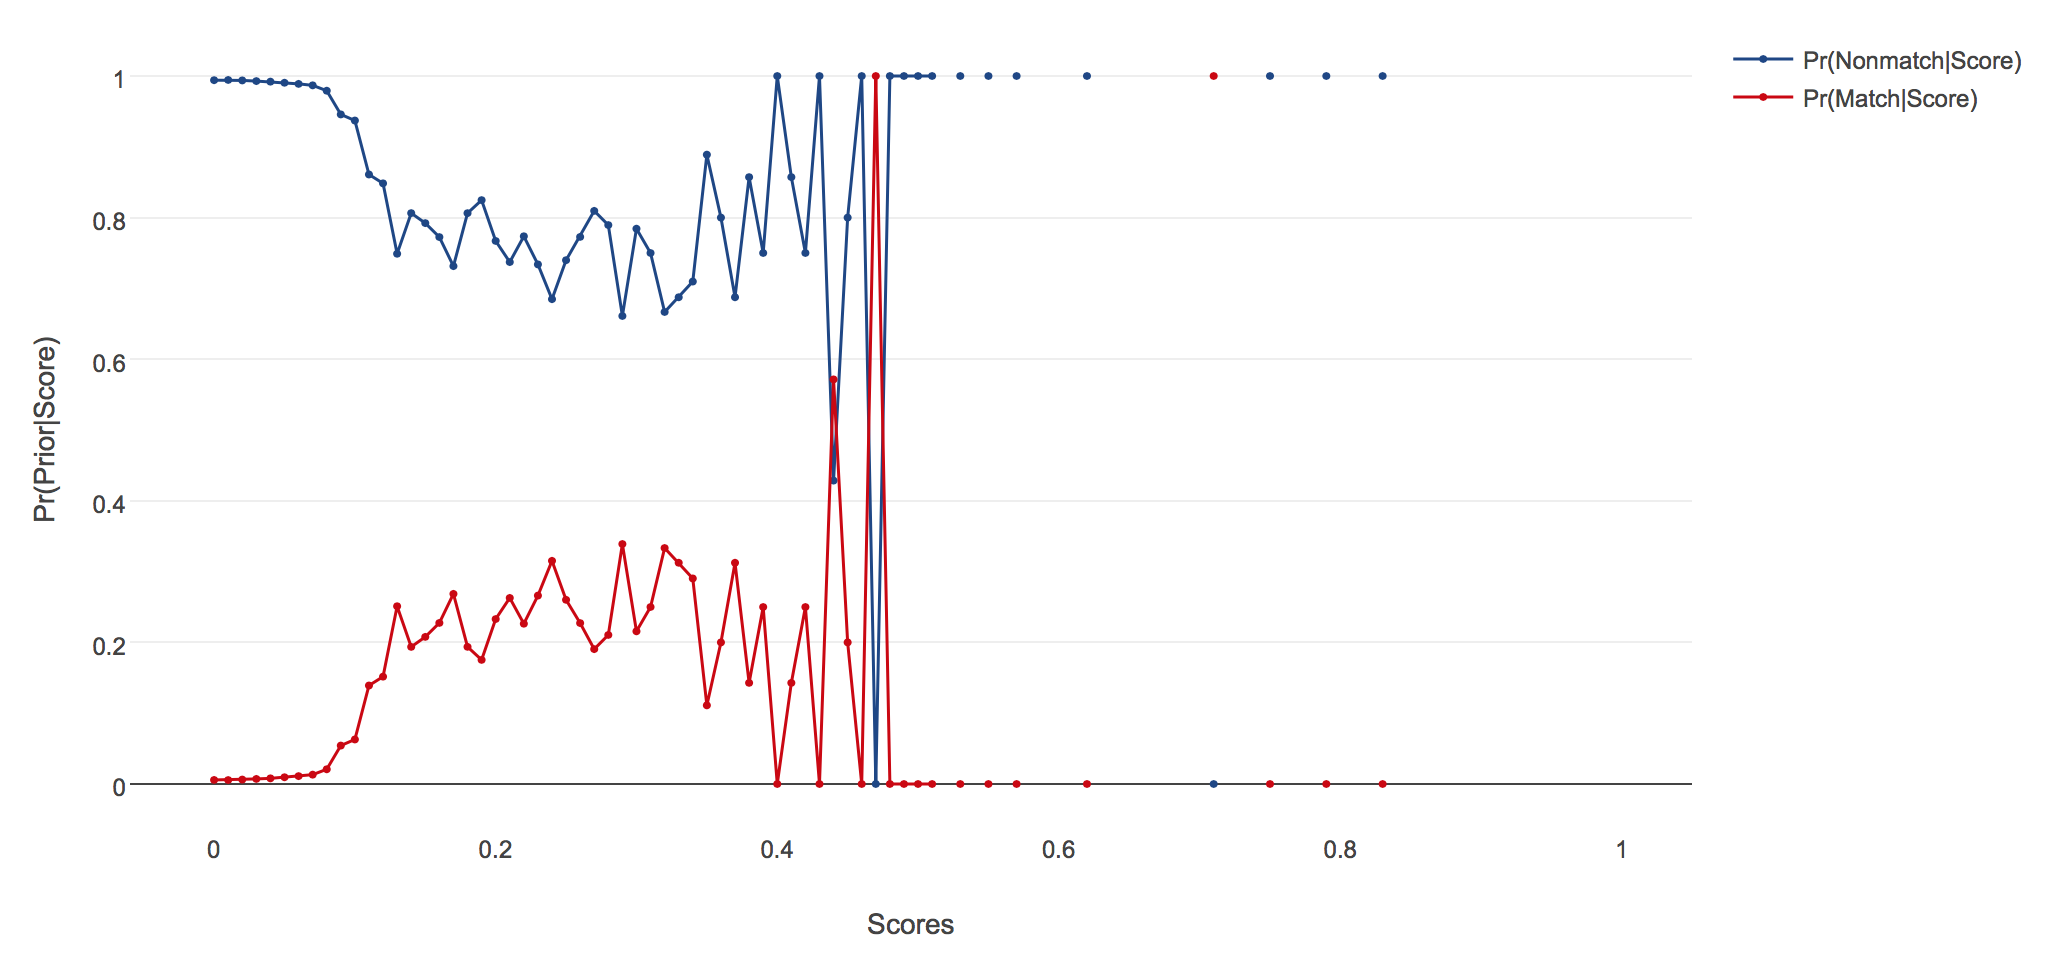
\includegraphics[width=0.95\textwidth]{dataset/grand/pms}
  \caption{Probability of matches/non-matches given score}
  \label{fig:grand_pms} %chktex 24
\end{figure}

\begin{figure}[ht]
  \centering
  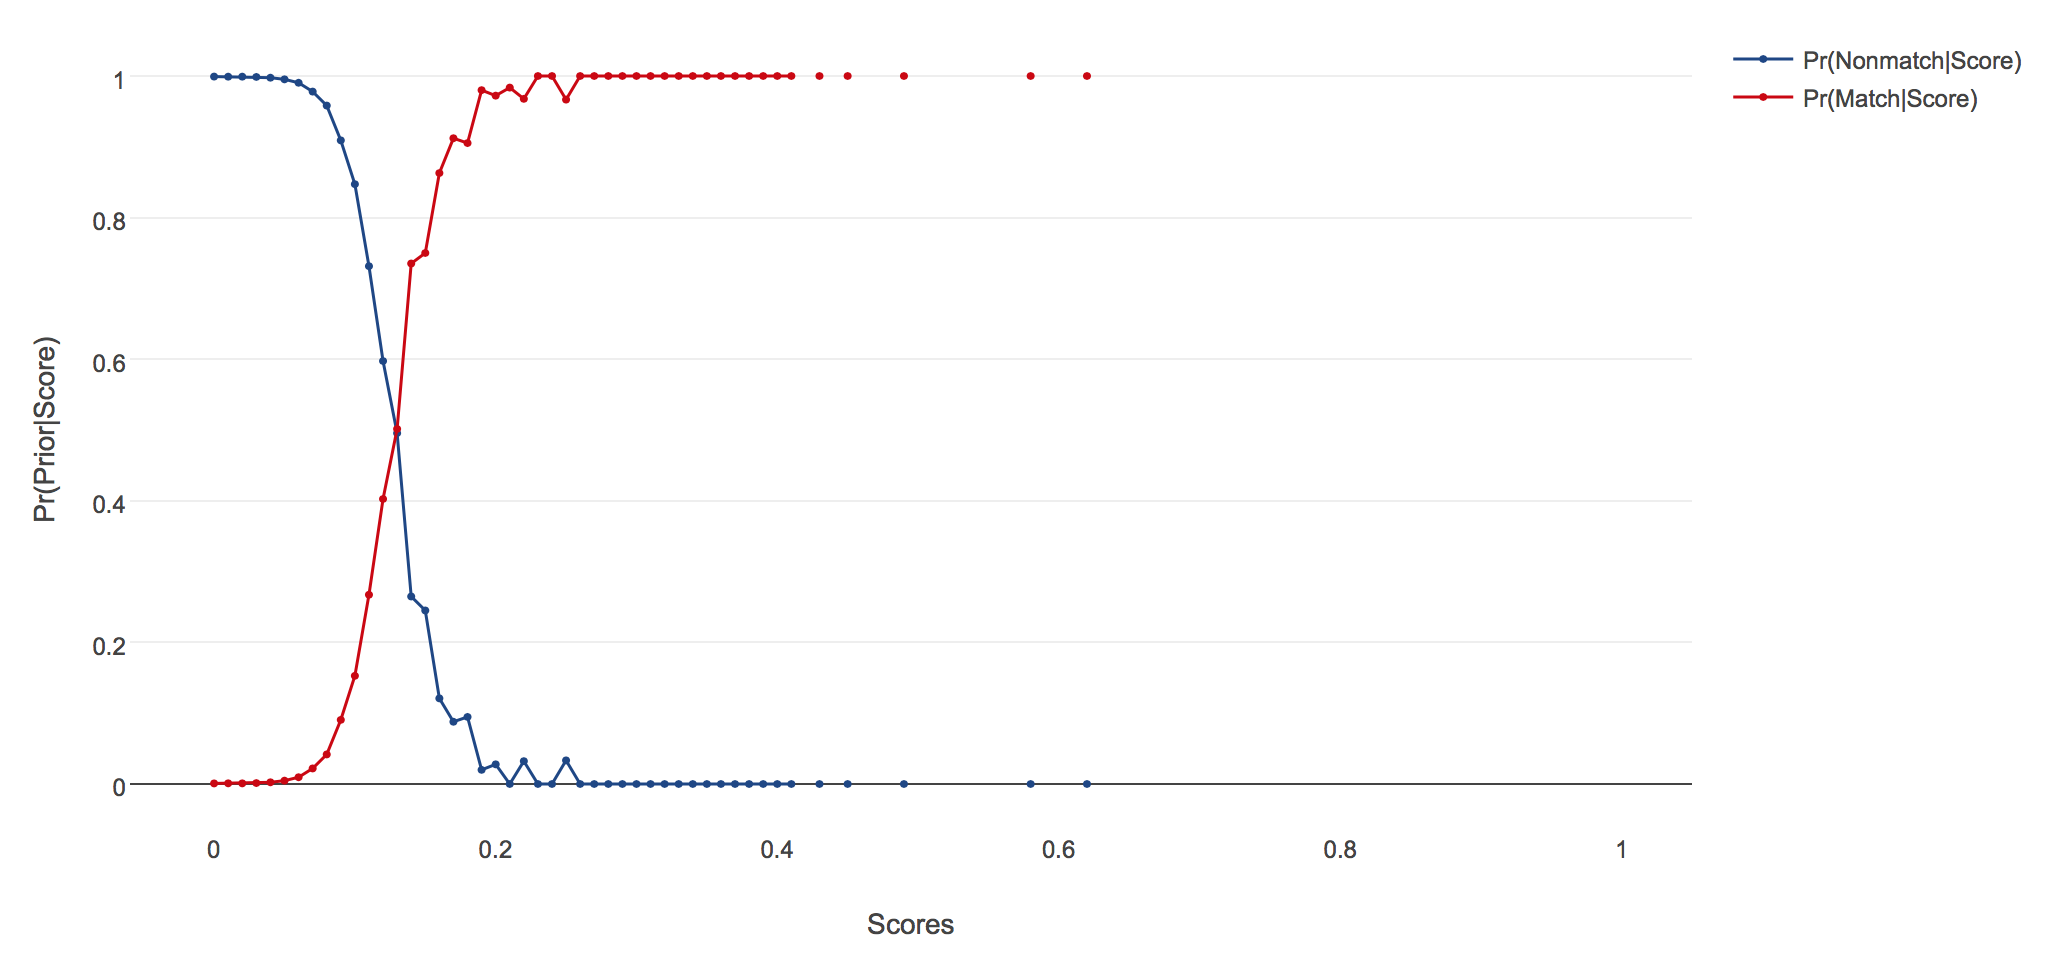
\includegraphics[width=0.95\textwidth]{dataset/otago/pms}
  \caption{Probability of matches/non-matches given score}
  \label{fig:otago_pms} %chktex 24
\end{figure}

\section{Adaptive Sampling Policies} % (fold)
\label{sec:sampling_policies}

Starting with a completely unknown pairs, we would like to first get the idea
of how the overall distribution looks like. As we have seen in
Chapter~\ref{chap:relevance_feedback}, the unbiased sampling policies, such as
Uniform, and AllScores, that broadly sample the data from the distribution seem
to form a set of good candidates.

Upon the retrieval of the general distribution, we would like to adaptively
utilize the known data to determine the optimal sampling site. We experiment
with sampling from the peak of the difference between the CDF of the score
given matches and non-matches using various sampling policies.

After we get the general picture of the distribution, we repeatedly reconstruct
the plot of the difference between the CDF of the score given matches and
non-matches, then uses normal sampling policy to overlay a Gaussian
distribution, with $\mu=$\texttt{peak\_of\_the\_CDF\_difference} and
$\sigma=0.3$, on the data. We continue each cycle by the sampling probability
distribution reconstruction, and sampling from the generated distribution.
Additionally, we also use Specific sampling policy to sample specifically at the
\texttt{peak\_of\_the\_CDF\_difference} to compare the performance with the
Normal sampling policy.

\section{Results}

\begin{figure}[h!]
  \centering
  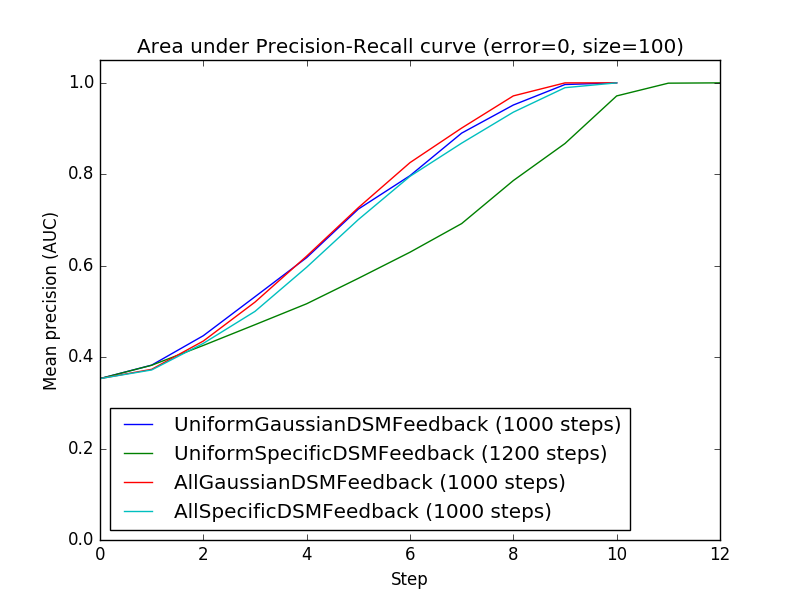
\includegraphics[width=0.8\textwidth]{otago}
  \caption{Mean Average Precision for the new sampling policies}
  \label{fig:otago_adaptive_aoc} %chktex 24
\end{figure}

The adaptive sampling policy seem to perform averagely well. The performance
does not differ from that of the other static sampling policies we have seen in
Chapter~\ref{chap:relevance_feedback}.

% section proposed_sampling_policy (end)
